%!TEX root = ../thesis.tex
\chapter{DemoWiz: Visualization for Software Demonstration}
\label{chapter_demowiz}
% \chapter{DemoWiz: Re-Performing Software Demonstrations for a Live Presentation}

Showing a live software demonstration during a talk can be engaging, but it is often not easy: presenters may struggle with (or worry about) unexpected software crashes and encounter issues such as mismatched screen resolutions or faulty network connectivity. Furthermore, it can be difficult to recall the steps to show while talking and operating the system all at the same time. An alternative is to present with pre-recorded screencast videos. It is, however, challenging to precisely match the narration to the video when using existing video players.

In this chapter, we introduce DemoWiz\footnote{This work was published at CHI 2014~\cite{Chi:2014:DRS:2556288.2557254}.}, a video presentation system that provides an increased awareness of upcoming actions through glanceable visualizations. DemoWiz supports better control of timing by overlaying visual cues and enabling lightweight editing. A user study shows that our design significantly improves the presenters’ perceived ease of narration and timing compared to a system without visualizations that was similar to a standard playback control. Furthermore, nine (out of ten) participants preferred DemoWiz over the standard playback control with the last expressing no preference.

%!TEX root = ../thesis.tex
\chapter{Introduction}
\label{chapter_introduction}

When attempting to accomplish unfamiliar, complicated tasks, people often look for tutorials to follow instructions. From performing daily tasks such as cooking and operating a machine, using software applications, to physical activities like sports and dance performance, each domain involves specific ``how-to'' knowledge with a certain degree of complexity~\cite{ryle1945knowhow}.
%
Instructions, which describe how a specific goal can be accomplished, are a tool for people to self-learn a task~\cite{Smith03iimanufacturer}. Studies have shown that visual instructions are cognitively favorable by people as they are easier to comprehend and remember than text information~\cite{Harrison:1995uh,mayer1996less,Heiser:2004:IVC:989863.989917}. In history, pictorial instructions have been created from the Middle Age to explain dancing or weapon operations~\cite{mijksenaar1999open}. It was found that the first use of letters in technical drawing for text referral was by Italian polymath Leonardo da Vinci. In 1737, French engineer de B{\'e}lidor~\cite{de1737architecture}'s diagrams were the first to apply arrows to indicate direction of movements (see Figure~\ref{fig:intro_arrows}).
%
From 1760, when the Industrial Revolution introduced mass production, instructions have been seen widely for various products and uses.

\begin{figure*}[h!]
  \centering
  \begin{minipage}{\textwidth}
  \includegraphics[width=\textwidth]{\intro/fig/arrows/arrows}
  \caption[Uses of motions arrows in visual instructions.]{Uses of motions arrows in visual instructions:
  %
  a) Year 1737: The first use of a motion arrow in an illustration explains the impact of water flow of a water wheel~\cite{de1737architecture},
  % http://www.buw-output-archiv.uni-wuppertal.de/ausgabe1/steinle/index-en.html
  %
  b) Year 2002: Similarly, arrows are used to explain the water flow and rotation of an undershot water wheel\footnote[1]{Original artwork by Daniel M. Short, ``Schematic diagram of an undershot water wheel'', licensed under CC BY-SA 2.5},
  % https://en.wikipedia.org/wiki/File:Undershot_water_wheel_schematic.svg
  %
  c) Year 2014: An animation visualizes the blood flow using motion arrows\footnote[2]{Video by Bioscience Credentials, ``Blood Flow in the Human Body'', \url{https://youtu.be/GwX41xm9esY}, licensed under CC BY 3.0}.
  }
  \label{fig:intro_arrows}
  \end{minipage}
\end{figure*}

Since the late 1990s, the advance in computer technologies has introduced more versatile instructional design. Instructions can now be created via software tools rather than hand drawing; they can include multimedia such as images and videos in several forms; they can be accessed through the Internet, as well as in hard copy.
%  the general purpose computers and the Internet
%
This advancement also enables consumers or end-users to document and share their domain knowledge~\cite{Lafreniere:2012tl}. As of today, popular tutorial sharing sites like Instructables has over 220,000 articles~\cite{InstructablesProjects}, wikiHow provides over 192,000 articles~\cite{wikiHowStatistics}, Food.com serves over 500,000 user-generated recipes with 125,000 photos~\cite{FoodComAbout}, and YouTube hosts over 285 million How-To videos\footnote{YouTube, \url{https://www.youtube.com/}, accessed June 2016}.
%
The variety of topics, content, and presentation styles provides learners more options to understand domain knowledge.
%
However, navigating a tutorial using existing tools remains inefficient for following step-by-step instructions. It can be challenging to observe details from text and images or find specific piece of information in a video through a timeline with conventional video players.
%
On the other hand, producing high-quality instructions that are easy to follow requires authoring expertise and a significant time investment. It involves several stages to design, record, and edit multimedia materials of a task using a variety of creation tools~\cite{Torrey:2007he,Tseng:2014:PVP:2598510.2598540,Muller:2009tw}.\\

The goal of this dissertation is to investigate interactive instructional design and develop computational tools that support the authoring process.
%
To contribute to computational methods of authoring user-generated instructions, two research questions that this work focuses on are:

\begin{itemize}
  \item How can authoring tools support domain experts in efficiently creating effective, high-quality instructions based on video-recorded demonstrations?
  \item How can new tutorial formats help authors better express their intent and help learners understand and follow the author's instructions?
\end{itemize}

This dissertation presents video-based computational approaches that enhance tutorial creation and consumption from author demonstrations.
We encode the current practices from professional authors into automatic algorithms and interactive techniques.
Our goal is to dramatically increase the quality of amateur-produced video instructions, which in turn improves learning for viewers who interactively navigate the content.
%
We will introduce five interactive systems that we develop to address these challenges. These tools cover both software applications (e.g., image manipulation tasks or browser navigation) and physical activities (e.g., Do-It-Yourself projects or dance movements) for recording, editing, and replaying instructional content.

% ---------------------------------------------------------------

\section{Challenges of Creating and Consuming Instructions}

Visual instructions are the dominant form of instructional design~\cite{mijksenaar1999open}. Cognitive load theory of multimedia learning suggests that learners process information using distinct channels, one for visual and the other for verbal formats~\cite{sweller1998cognitive,sweller1988cognitive,paas2003cognitive}. It was found that learners performed better when received a pictorial summary of a scientific system than those who received the full text alone or the full text with the summary~\cite{mayer1996less}.

Among all the multimedia support, videos are a common form to present instructions. We suspect that the great popularity of videos is due to the following reasons:
%
First, consumer devices and software have become affordable for authors to quickly record activities and later share via online platforms at minimum cost.
%
% ** describe the difficulties of making knowledge "explicit", esp. for actions and motions
Second, videos can be an efficient medium to document activities. Transferring know-how concisely and effectively to the audience is challenging. It especially requires efforts when a task involves \emph{tacit knowledge}, which is a kind of knowledge that is difficult to articulate in a written or verbal form~\cite{polanyi1958personal, Klemmer:2006:BMF:1142405.1142429}. Examples of tacit knowledge include dancing, riding a bike, or driving nails with a hammer. Dancers can perform movements fluently with music. If they are asked to focus on the composite pieces, such as the arm and foot actions or rhythm, they might get confused and fail to express the entire movement~\cite{polanyi1958personal}. Very often, recording a video eases the difficulties of describing the entire activities in an explicit form.
%
This leads to another motivation that videos also provide an effective channel to convey ideas with adequate amounts of details. Learners can visually observe the exact actions in a video as if an expert were coaching in person~\cite{Kuznetsov:2010:REA:1868914.1868950}.

However, while videos are easy to produce, they can include a lot of unnecessary footage. Inevitable content such as pauses, mistakes, and long repetitive actions makes it difficult for learners to focus on the most important steps and actions. A lot of authoring effort commonly goes into extracting footage, applying visual effects, and adding subtitles and annotations.
%
In addition, even with a well-edited video, navigating using a conventional video player remains inefficient. Learners with various needs could have a hard time skimming to an interesting moment or perceiving high-level overviews. Alternatively, a pictorial summary or static step-by-step tutorials presented with text and images can effectively guide knowledgeable learners through familiar tasks.

% The goal of this dissertation to develop video-based recording, editing, and playback tools are optimized for creating and consuming instructional demonstrations. I combine the advantage of ubiquitous video recording with the benefits of video and structured tutorial formats. I aim to dramatically increase the quality of amateur-produced video instructions, which in turn improves learning for viewers who interactively navigate the content.

% ----- MixT ----- %

\subsection{New Tutorial Formats}

Both static and video tutorials have strengths, but neither format alone is well suited for all learning needs that learners may have.
%
To combine the benefits, we design a new instructional presentation called \emph{MixT} (mixed-media tutorials) that improves learners' success in following instructions (see Figure~\ref{fig:mixt_intro}).
%
MixT presents step-by-step static instructions and includes in-place video clips for each operation.
%
With MixT, learners can quickly scan forward and backward on a web page to obtain an overview of a task. Embedded videos help them understand continuous, complex manipulation, such as brushing on a canvas and adjusting control points.
%
MixT's playback UI allows learners to interactively control \emph{when} to see images or videos, and \emph{how} to render videos.
%
Video editing techniques are applied to emphasize instructions, including cropping salient screen regions and highlighting interaction.
%
In our within-subject experiment, MixT successfully reduced numbers of errors and attempts made by learners when following image manipulation tasks.
% To demonstrate , MixT captures screencast video and operation events of a software demonstration.

\begin{figure*}[t]
  \centering
  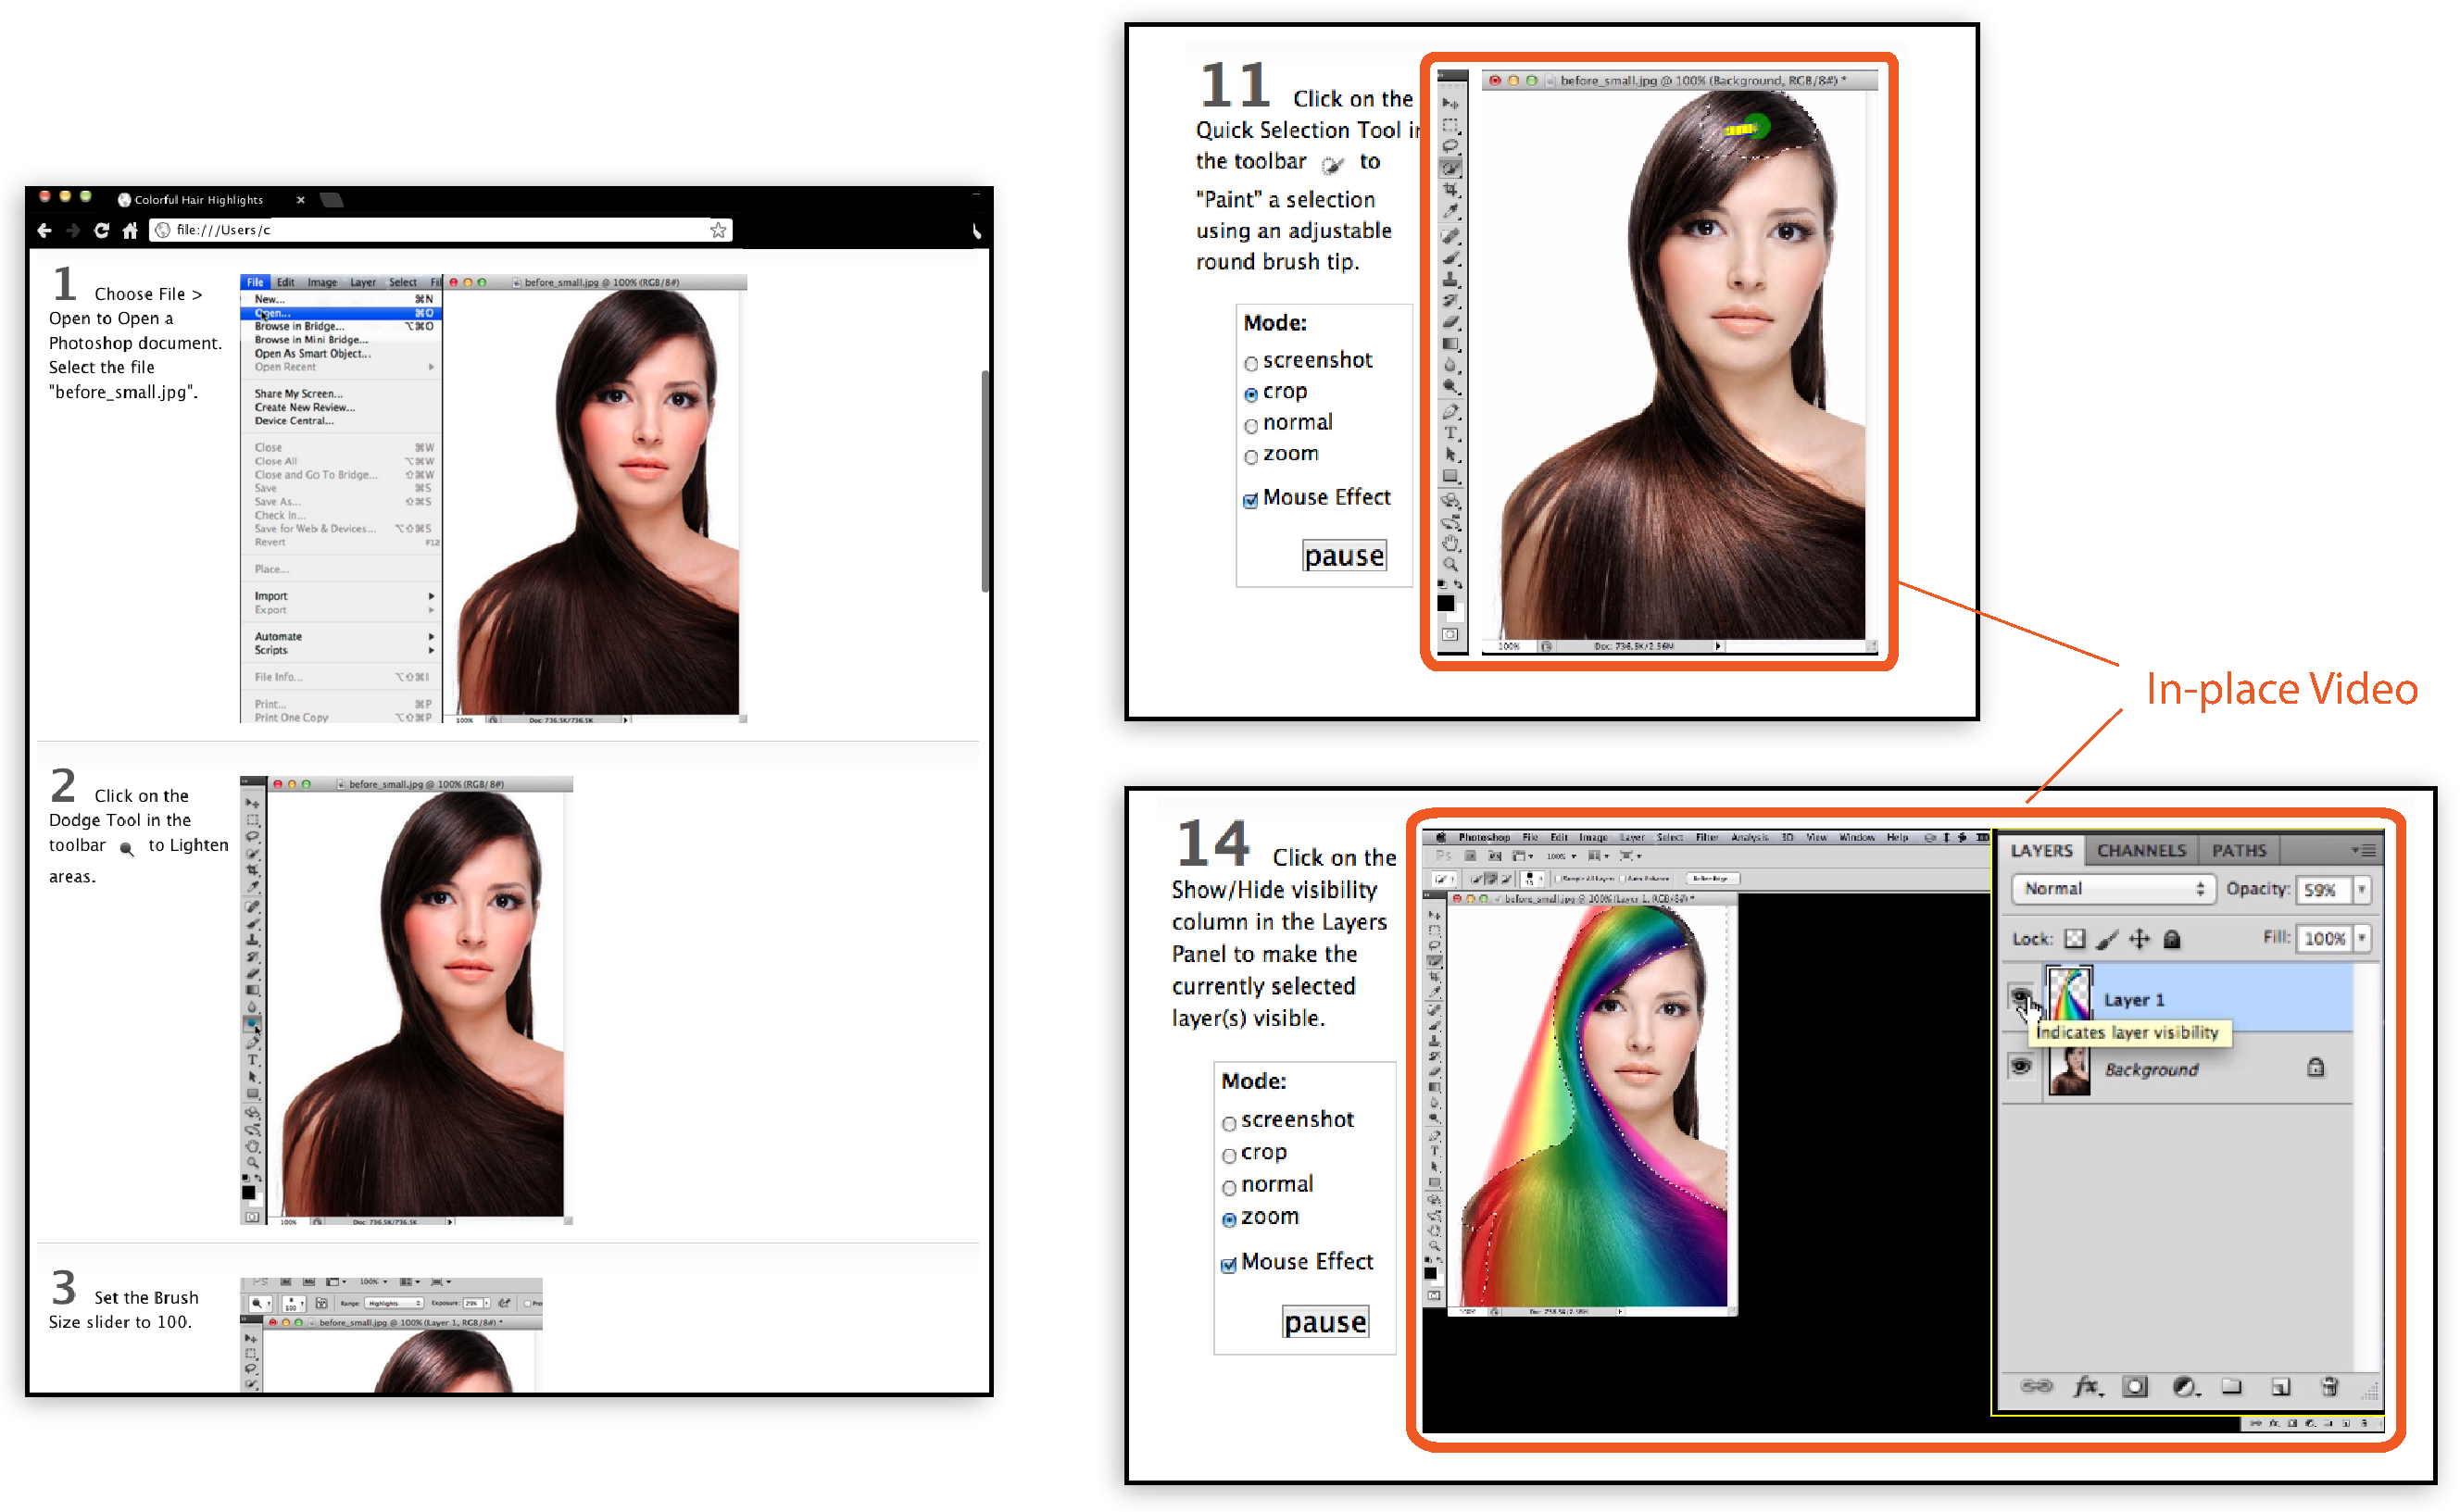
\includegraphics[width=0.8\textwidth]{\intro/fig/mixt_intro}
  \caption{MixT generates step-by-step tutorials (left) that contain static and video information from task demonstrations. Videos are automatically edited and offer different views (right) to highlight the most relevant screen areas for a step. Visualizing mouse movement helps learners understand a complex action.}
  \label{fig:mixt_intro}
\end{figure*}

% ----- DemoWiz ----- %
MixT offers a novel way of navigating instructional content with a combination of static step-by-step and embedded video presentations. If an author wants to narrate over a video recording to illustrate a demo, it can be challenging to pace oneself at the suitable timing without expecting \emph{when} and \emph{what} action is taking while a video is playing.
%
We design \emph{DemoWiz}, a system that augments a screencast video with visualizations (Figure~\ref{fig:demowiz_intro}). By logging the input events of a software demonstration, DemoWiz overlays glyphs to visually guide viewers to the next action along with the time remaining before the action occurs. This enables viewers to anticipate the video content rather than react to it.
%
Our study showed that fewer anticipation errors and narration delays were made with DemoWiz.

\begin{figure*}[t]
\centering
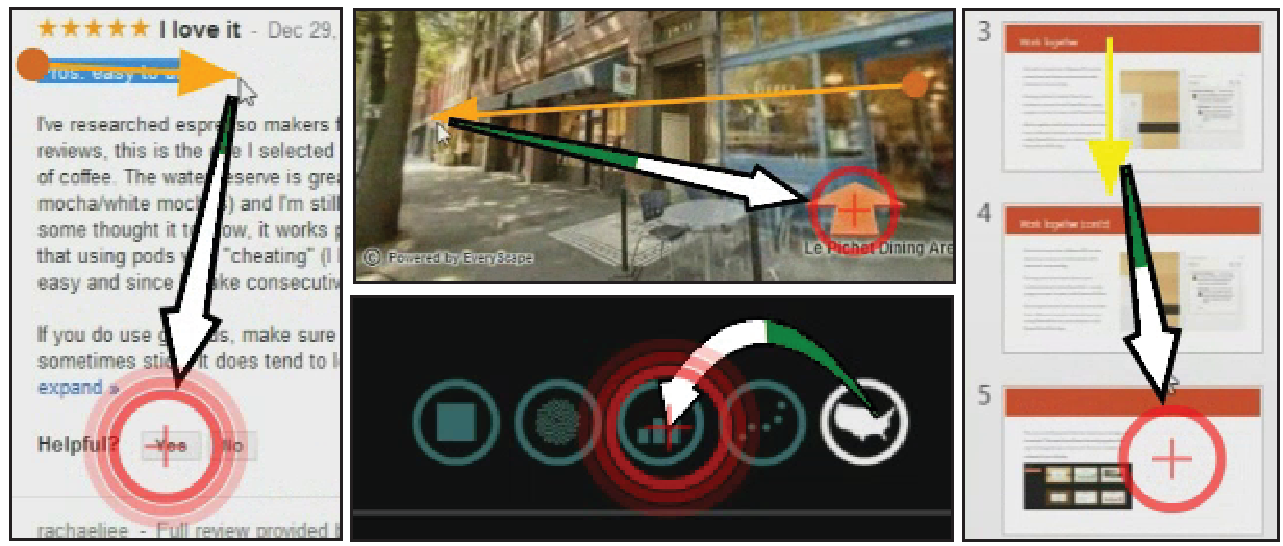
\includegraphics[width=0.7\columnwidth]{\intro/fig/DemoWiz}
\caption{DemoWiz visualizes input events in a screencast video to help viewers anticipate the upcoming event for following a software demonstration.}
\label{fig:demowiz_intro}
\end{figure*}

\subsection{Tutorial Generation from Software Demonstration}

While new tutorial formats are shown to be useful, manually creating instructions can be extremely time- and effort-consuming. In response, we design computational methods to automate the creation process from an author demonstration. MixT and DemoWiz capture screencast video and input device events from a demonstration of a task in a software application. MixT also records application commands for video analysis. Computer vision and visualization techniques are integrated to segment a video into steps, extract salient information, and add visual highlights.
%
In addition, DemoWiz supports an editing phase where authors can adjust the timing of events in a video. Playback speed of recorded actions can be modified or skipped via an editing UI. Our studies showed that our algorithms for step segmentation, event detection, and visualization were effective (\textless8\% error rate in MixT and 0\% in DemoWiz).

\subsection{Interactive Tutorial Authoring from Physical Demonstration}

% ----- DemoCut ----- %

Moving beyond software applications, support for authoring instructions of tasks that take place in the physical world is lacking. Activity recognition remains an open research question, and making authoring decisions during a demonstration can be difficult.
%
To address this problem, we first look into Do it yourself (DIY) project tutorials, which help people learn knowledge and skills to complete a task independently.
%
We developed \emph{DemoCut}, a semi-automatic video editing system that improves the quality of amateur instructional videos for physical tasks (Figure~\ref{fig:democut_intro}). DemoCut asks authors to describe key ``moments'' in a recorded demonstration video using a set of markers. Based on the annotations, our system analyzes the audio and visual activities to automatically organize the video into meaningful segments. Editing decisions are applied to support both \emph{temporal effects} that increase playback speed or skip segments, as well as \emph{visual effects}, such as zooming, subtitles, and visual highlights. A playback interface allows authors to quickly review and edit the automatically generated effects.
%
Our studies showed that video tutorials created by DemoCut in five DIY domains were concise in terms of video length and descriptive instructions with low effect error rates.

\begin{figure*}[t]
  \centering
  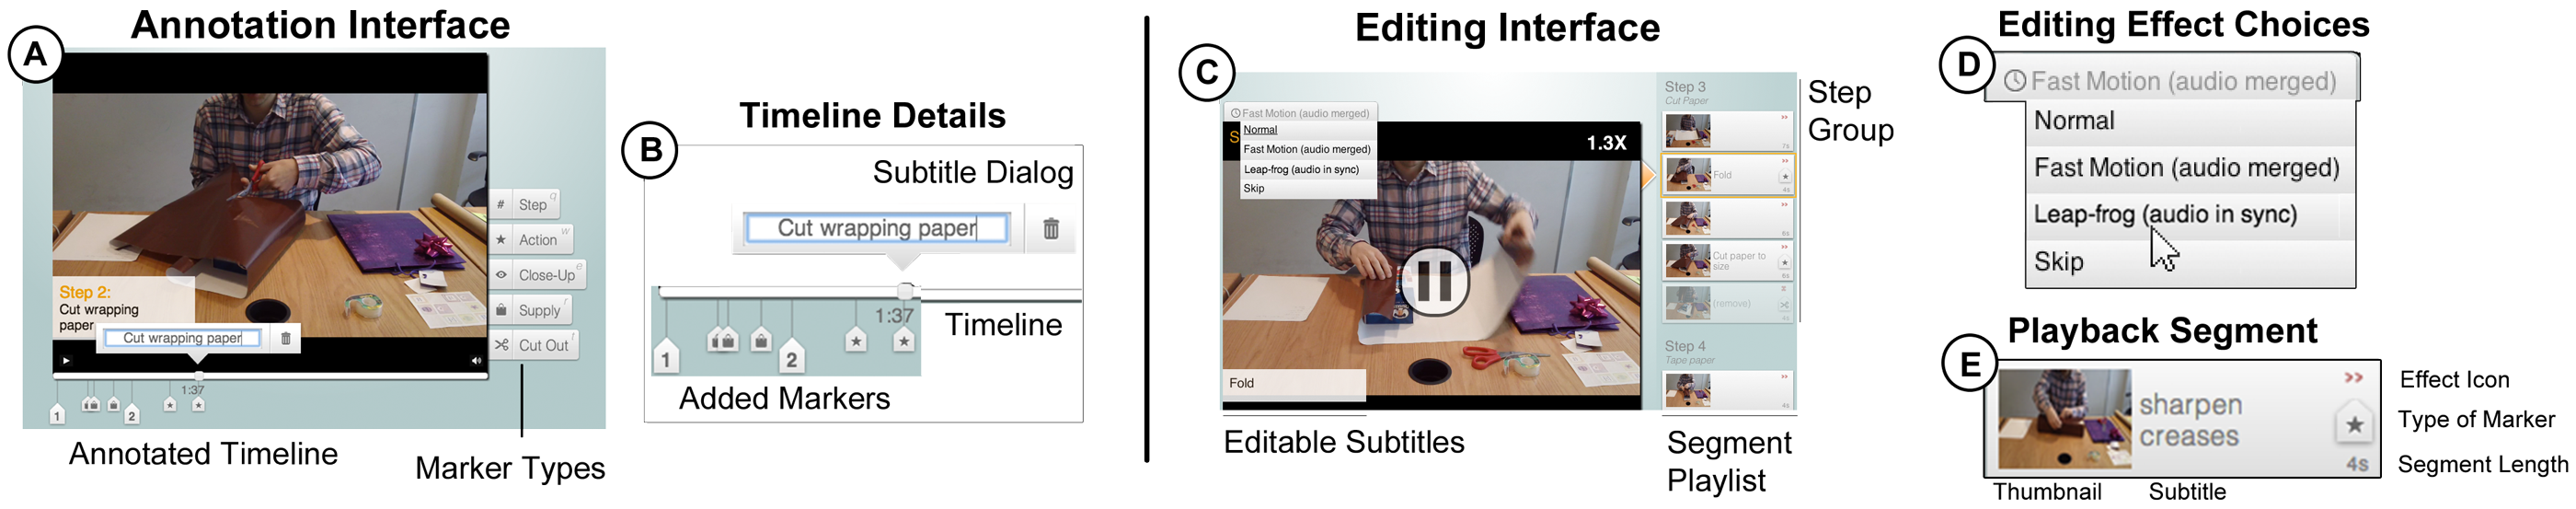
\includegraphics[width=\textwidth]{\intro/fig/DemoCut}
  \caption{DemoCut asks authors to mark key moments in a recorded video of demonstration using a set of marker types. Based on marker information, the system uses audio and video analysis to automatically organize the video into meaningful segments and apply appropriate video editing effects, which can be modified via a playback UI.}
  \label{fig:democut_intro}
\end{figure*}

% ----- Kinectograph ----- %
Through the process of designing DemoCut for automatic DIY video editing, we observed that for tasks that require larger space and more movements, instructors often have to adjust the position and viewing angle of a camcorder. Some authors choose to set up multiple cameras and later select the best shot from video streams, while some invite another person who controls the camcorder during a demonstration.
%
To enable authors to record their demonstration without acquiring additional cameras or cameraman, we design \emph{Kinectograph}, a video recording device with a single camera that automatically tracks and follows specific body parts, e.g., hands, of an instructor in a video (see Figure~\ref{fig:kinectograph_intro}). It utilizes a Kinect depth sensor to track skeletal data and adjusts the camera angle via a 2D pan-tilt gimbal mount. Authors can freely move around in space to demonstrate a task and monitor real-time video preview through a tablet application.

\begin{figure}[!t]
  \centering
  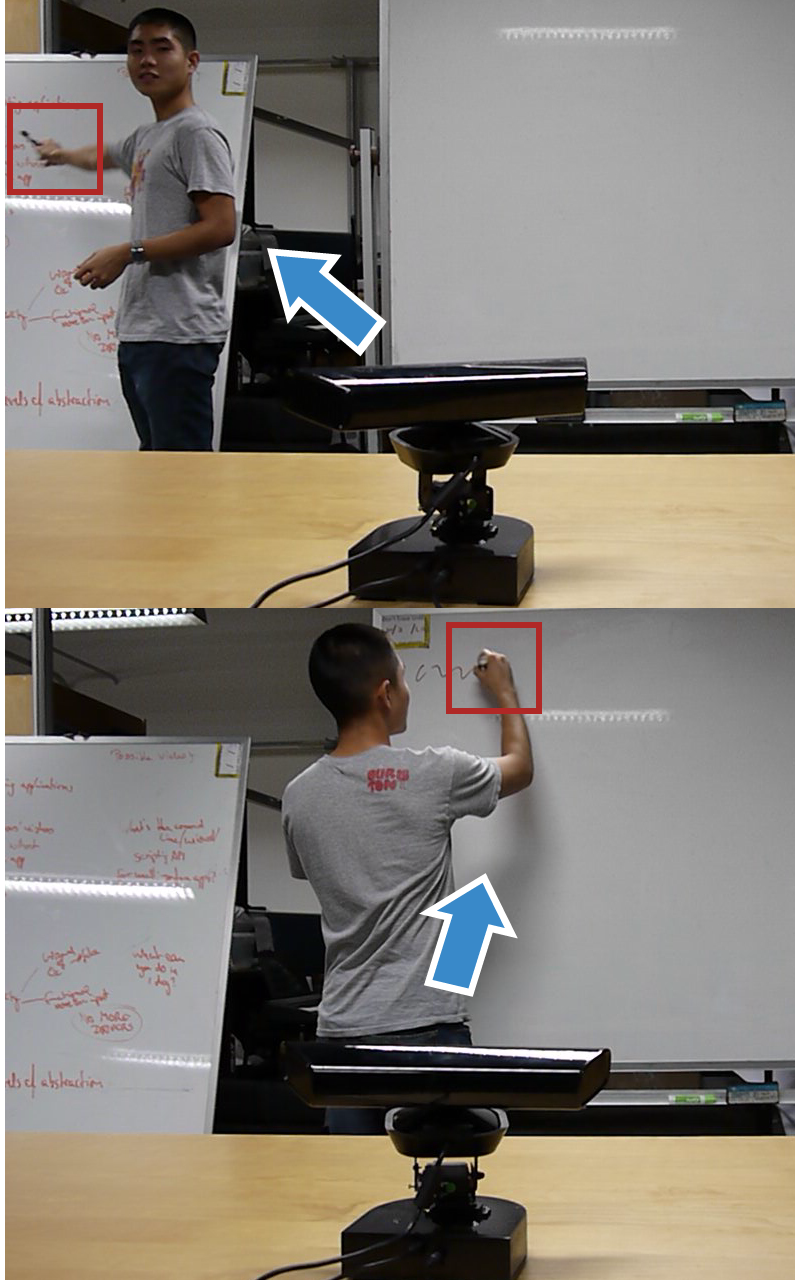
\includegraphics[width=0.65\columnwidth]{\intro/fig/Kinectograph}
  \caption{Composed of a Kinect camera to track author movement and a motorized dock to pan and tilt the camera, Kinectograph allows the author (or their hand) remains centered in the recorded video in real-time.}
\label{fig:kinectograph_intro}
\end{figure}

% ----- DemoDraw ----- %

The successful experiences supporting motion-based recordings motivated me to apply our demonstration-based approach to a domain that is entirely driven by movements. In sports, dance performance, and body gesture interfaces, movement instructions are often conveyed with drawings of the human body annotated with arrows or stroboscopic effects~\cite{cutting_representing_2002}. However, current practices require authors to manually sketch or trace subjects from photographs, which is time-consuming and difficult to make changes once created.
%
We design \emph{DemoDraw}, a system that generates concise illustrations from author demonstration (see Figure~\ref{fig:demodraw_intro}). With DemoDraw, an author records one or more motions by physically demonstrating in front of a Kinect sensor. In a multi-modal Demonstration Interface, DemoDraw segments speech and 3D joint motion into a sequence of motion segments, each characterized by a key pose and salient joint trajectories. Based on this sequence, a series of illustrations is automatically generated using a stylistically rendered 3D avatar annotated with arrows to convey movements. Once a suitable sequence of steps has been created, a Refinement Interface enables fine control of visualization parameters.
%
In a three-part evaluation, our results show 4 to 7-step illustrations can be efficiently created in 5 or 10 minutes on average.

\begin{figure}[t]
  \centering
  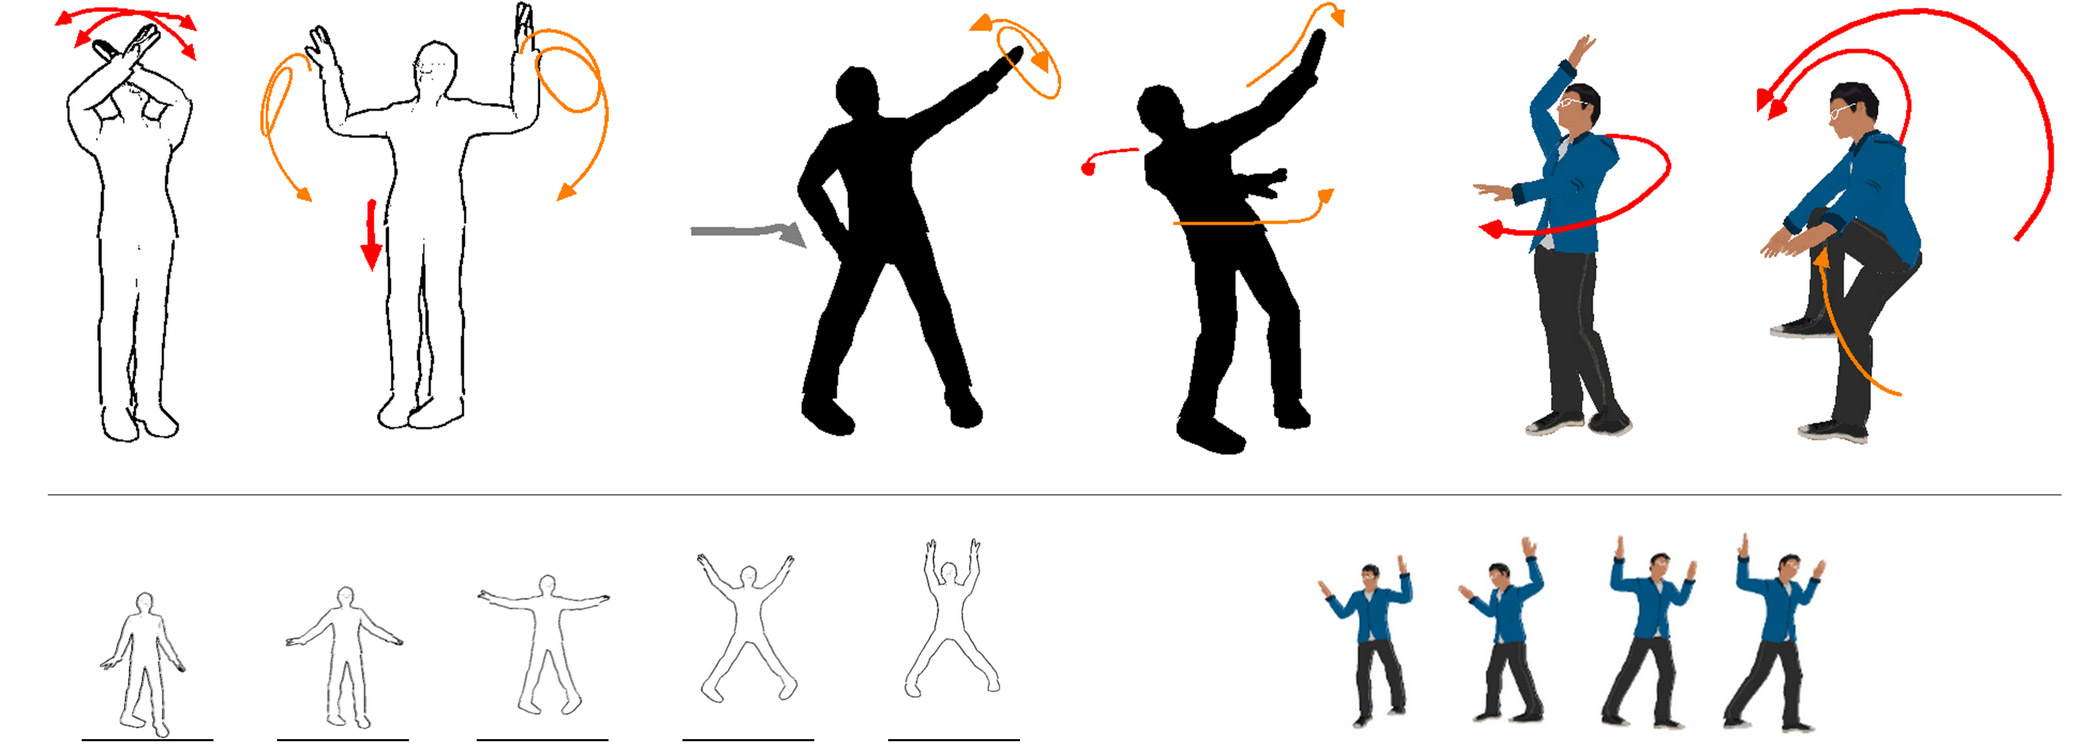
\includegraphics[width=\columnwidth]{\intro/fig/DemoDraw}
  \caption{DemoDraw's multi-modal approach enables authors to capture motion, verify results, and re-perform portions if needed to generate step-by-step motion illustrations.}
  \label{fig:demodraw_intro}
\end{figure}

% ---------------------------------------------------------------

\section{Thesis Contributions}

Overall, our video-based approaches consider key events or moments that are important to a learner. This information can be derived from software event logs or human annotation of physical tasks when automatic recognition remains challenging. Based on the metadata and video streams, we propose automatic methods to generate concise instructions for two task domains, software applications and physical tasks (see Figure~\ref{fig:space}). Our approaches support authors from recording demonstrations to editing and reviewing system-generated instructions. Interactive controls are available in different stages via desktop or multi-modal interfaces.
%
We demonstrate a series of systems that consider production stages of tutorial creation and learning. We present the rationale and technical challenges of these interactive system designs. Each system is evaluated both quantitatively and qualitatively to study the usability in authoring and learning.

\clearpage
The contributions of this dissertation include:

\begin{itemize}
\item New instructional formats that consider the learning needs from several domains, including software applications and physical activities.
\item Multi-modal interaction techniques for novice or amateur authors to create effective instructions by demonstration.
\item Automatic or semi-automatic approaches using video and audio analysis that includes authors in the loop to produce high-quality instructions.
\end{itemize}

\begin{figure}[t!]
  \centering
  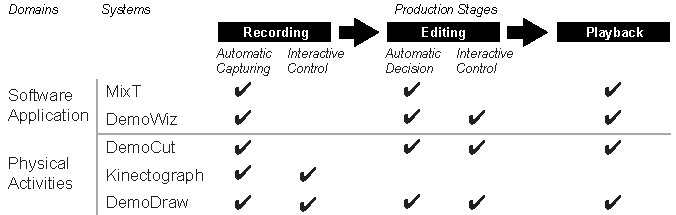
\includegraphics[width=0.9\columnwidth]{\intro/fig/space}
  \caption{A design space of the creation and consumption process for tutorials. It involves three phases of recording, editing, and playback in either software domain or a physical world. This dissertation proposes a series of systems that focus on various aspects in this design space.}
  \label{fig:space}
\end{figure}

% ---------------------------------------------------------------

\section{Overview}

The rest of this dissertation is structured as follows:
%
In Chapter \ref{chapter_background}, we define terminology used in instruction creation and consumption process based on literature. We review studies on why people rely on tutorials in general, how the formats of instructions matter, and the current practices of authoring instructions.
%
In Chapter \ref{chapter_related_work}, we review the literature on research and technologies used in supporting activities of authoring and consuming instructions.

We presented two systems that generate interactive tutorials for software applications.
% MixT
In Chapter \ref{chapter_mixt}, we present our study on how a new tutorial format supports learners in following step-by-step instructions with mixed media, including static text, images, and video clips. We introduce our creation tool called MixT, which automatically generates such new tutorial format from a software demonstration.
% DemoWiz
Chapter \ref{chapter_demowiz} introduces DemoWiz, a system that assists viewers in capturing the timing of input events in a screencast demo video. DemoWiz supports recording, editing, and reviewing stages in a production process with an authoring and playback UI.

Then, we introduced three systems designed for real-world tasks that involve physical demonstrations.
% DemoCut
In Chapter \ref{chapter_democut}, we present a semi-automatic tool for DIY video editing. Our system, called DemoCut, provides two authoring interfaces, annotation and editing, that enable authors to mark a demo video and review and modify the automatically edited results. The design is based on an fundamental understanding of DIY activities.
% Kinectograph
In Chapter \ref{chapter_kinectograph}, we focus on a recording device that automatically follows a demonstrator for filming instructional videos. The Kinectograph system tracks an author's position and body parts and provides an authoring interface for real-time camera control.
% DemoDraw
Finally, in Chapter \ref{chapter_demodraw}, we introduce a multi-modal approach for authors to generate motion illustrations by physically demonstrating the movements. DemoDraw is a system that segments speech and 3D joint motion into a sequence of motion segments and renders effective illustrations. Two authoring interfaces enable authors to navigate, re-perform, and edit visualization parameters.

% Conclusion
Throughout this dissertation, we discuss how our video-based approaches increase the quality of amateur-produced video instructions. Chapter \ref{chapter_conclusion} concludes our work on tutorial creation and consumption in both software and physical instructions. New directions for future research on interactive tutorials are proposed.

% ---------------------------------------------------------------

\section {Prior Publications}

This dissertation is based on papers published in previous ACM conference proceedings: the MixT system was published at UIST 2012~\cite{Chi:2012:MAG:2380116.2380130}, DemoWiz at CHI 2014~\cite{Chi:2014:DRS:2556288.2557254}, DemoCut at UIST 2013~\cite{Chi:2013:DGC:2501988.2502052}, and Kinectograph at CHI 2013~\cite{Cheng:2013:BCC:2468356.2468568}; DemoDraw will be published at UIST 2016~\cite{Chi:2016:DemoDraw}.

While I am primary author on all publications and led the described projects, this research could not have been completed without my advisor Bj\"orn Hartmann and my collaborators that I have been fortunately to work with. Specifically, Dr. Mira Dontcheva and Dr. Wilmot Li at Adobe Research provided valuable guidance on three projects (MixT, DemoCut, and DemoDraw); Dr. Steven M. Drucker and Dr. Bongshin Lee at Microsoft Research guided the DemoWiz project with their expertise on visualization; Professor Daniel Vogel at University of Waterloo greatly contributed to the DemoDraw project. A group of MS and undergrad students at UC Berkeley and Adobe contributed to implementation, design, and user study in the projects, including Sally Ahn and Amanda Ren in MixT, Joyce Liu and Jason Linder in DemoCut, and Derrick Cheng and Taeil Kwak in Kinectograph.

% We are all natural performers. Humans are proficient at demonstrating how to perform a task in action. However, articulating knowledge into a written or structured form can be extremely difficult. From dancing, repairing a machine, to operating software applications, it remains a challenge how everyday activities can be efficiently captured for a remote learner to understand.

%!TEX root = ../thesis.tex

\chapter{Related Work}
\label{chapter_related_work}

While existing practices require tutorial authors to create instructions manually, HCI and Computer Graphics communities have introduced novel technologies for authoring tutorials, including automatic generation methods and interactive editing tools.
%
In this chapter, I survey state-of-the-art techniques for generating instructions for both software applications (Section \ref{related_software}) and physical tasks (Section \ref{related_physical}).
%
Furthermore, existing instructions are mainly offered in the forms of conventional media, such as static tutorials (print-outs or web) or videos. With software systems, \keyword{interactive tutorials} have been introduced for learners to interactively review instructional content. I will discuss various forms of such kind of instructions by prior research, which leads to a discussion on the remaining gaps in tool support for creating and navigating instructional content.

% -------------------------------------------

\section{Instructions for Software Applications}
\label{related_software}

\subsection{Workflow Capturing and Tutorials}

Revealing operation history has shown to be effective in presenting software instructions. Operational events can range from low-level, application agnostic input device events (e.g., mouse actions, cursor movements, or keyboard strokes) to higher level, application-dependent information (e.g., menu selections or UI component changes).
%
Researchers have investigated automatic approaches that capture and visualize these types of events. Nakamura and Igarashi~\cite{Nakamura:2008:ASV:1449715.1449721} proposed a capturing and rendering system independent to GUI applications. Their system logs mouse events of a software demonstration process, including mouse moving, dragging, and clicking. Operations are rendered as markers and arrows on screenshot images to present the linear event history (see Figure~\ref{fig:related_events} top).
%
Grabler \ea{}'s approach~\cite{Grabler:2009jj} further analyzes the application context, including facial features and outdoor scenes, and annotates software screenshots with arrows, bounding boxes, and call-outs (see Figure~\ref{fig:related_events} bottom). In addition to annotated images, their system generates textual description from templates, such as \iquote{Select the \textbf{path tool} from the \textbf{toolbar} to \textbf{create and edit paths}.} The generated text and rendered images of operations are presented as a step-by-step tutorial, which is currently available as a Photoshop plug-in\footnote{Adobe labs. Tutorial Builder. \url{http://labs.adobe.com/technologies/tutorialbuilder/}}.

Demonstration-based approaches for generating instructions have been also applied to applications that involve more complicated manipulations or gestures, including 3D mesh construction~\cite{Denning:2011fy} and mobile apps~\cite{Wang:2014:EAC:2556288.2557407}.
%
Beyond logging events from recording a user demonstration, researchers have shown that workflows and software content can be captured automatically using application logs \cite{Grossman:2010jz,Grabler:2009jj,Pongnumkul:2011ju} or computer vision from analyzing desktop regions~\cite{Yeh:2009dh,Chang:2011vd} and existing screencast videos~\cite{Banovic:2012kd}.

\begin{figure*}[t!]
  \centering
  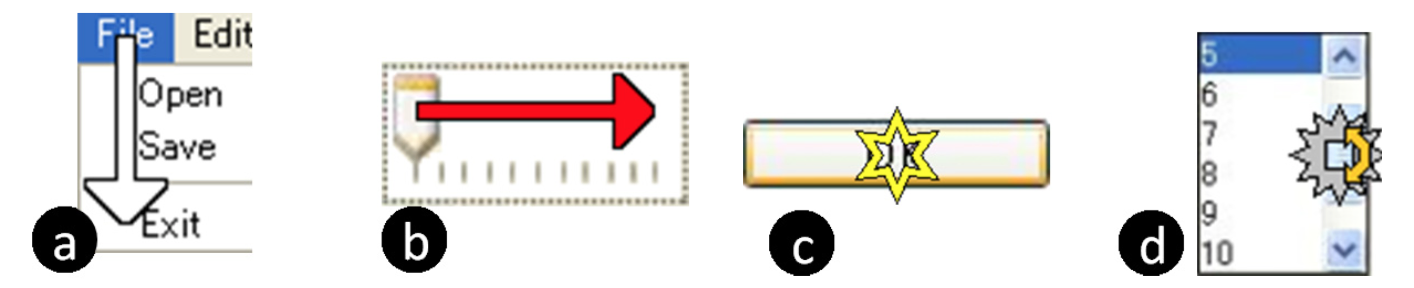
\includegraphics[width=0.6\textwidth]{\background/fig/software_viz/Nakamura_and_Igarashi}
  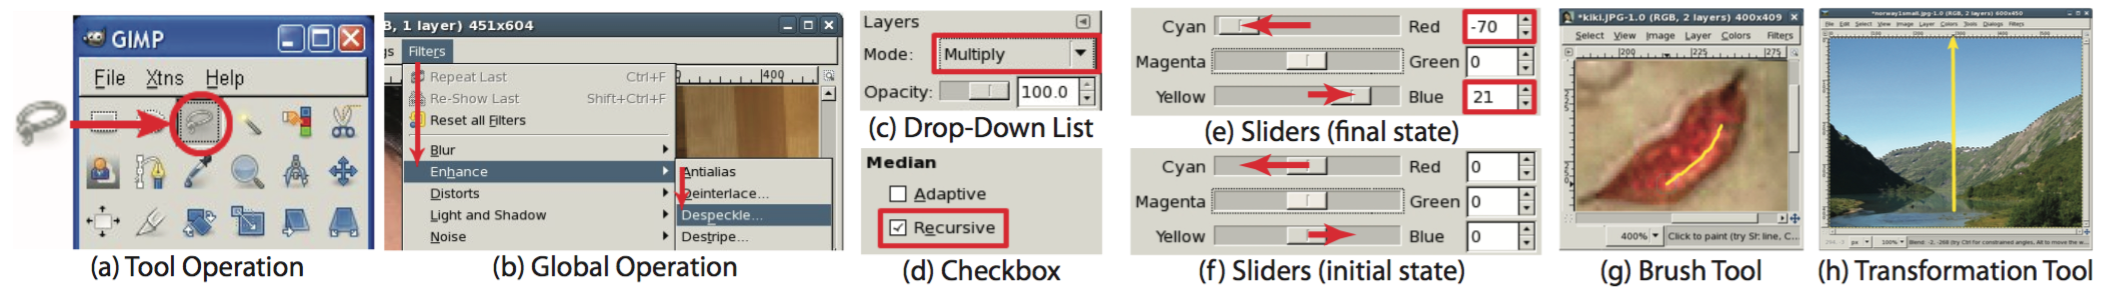
\includegraphics[width=\textwidth]{\background/fig/software_viz/Grabler}
  \caption{Example screenshots that visualize mouse operations are automatically rendered, including (top) mouse move, drag, click, and wheel (a-d) by Nakamura and Igarashi~\cite{Nakamura:2008:ASV:1449715.1449721} and (bottom) application-specific operations (a-b), parameters (c-f), and manipulations (g-h) by Grabler \ea{}~\cite{Grabler:2009jj}.}
  \label{fig:related_events}
\end{figure*}

To compare operation effects and workflows, other effective visualization approaches include showing a list of ``before'' and ``after'' thumbnails, video clips, and event timeline \cite{Grossman:2010jz} and creating a union graph of operations \cite{Kong:2012:DTR:2207676.2208549} (see Figure~\ref{fig:related_comparison}).

\begin{figure*}[t!]
  \centering
  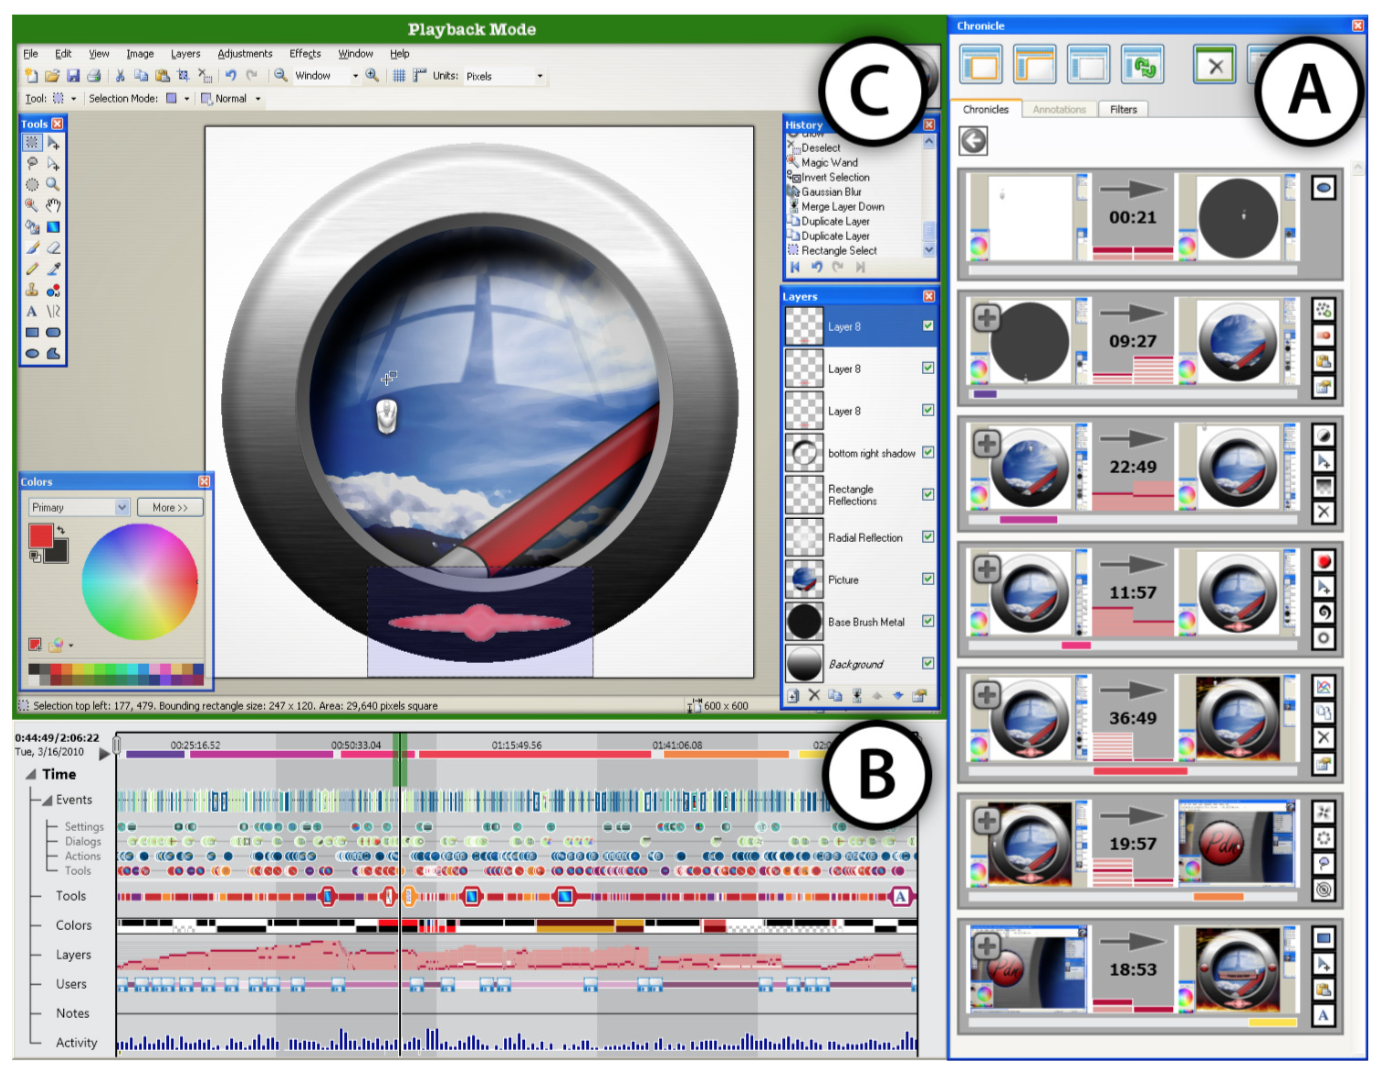
\includegraphics[width=0.4\textwidth]{\background/fig/software_viz/Grossman}
  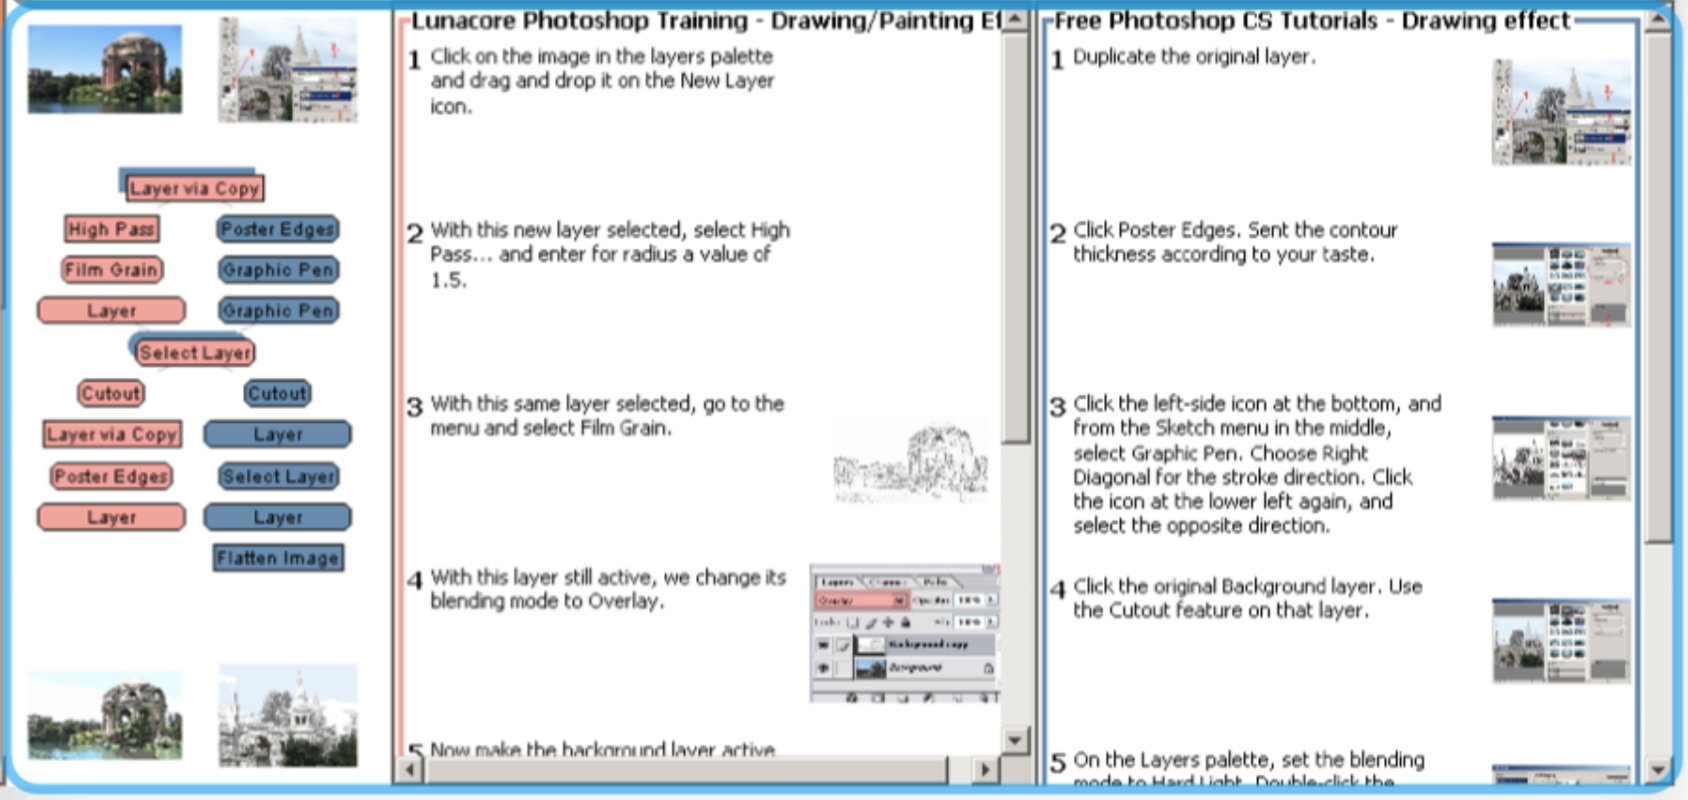
\includegraphics[width=0.55\textwidth]{\background/fig/software_viz/Kong}
  \caption{Instructional systems that help learners compare effects and similar tutorials using: (left) before and after images (a) and event timeline (b) by Grossman \ea{}~\cite{Grossman:2010jz} and (right) operation union graph by Kong \ea{}~\cite{Kong:2012:DTR:2207676.2208549}.}
  \label{fig:related_comparison}
\end{figure*}

% -------------------

\subsection{In-Application Support}

The above systems introduce innovative ways of providing informative screenshots or representations for learners to review workflows. However, reviewing these materials is often separated from operating a software application. Learners might have to switch between context of interacting an application and reading instructions, which could introduce a gap of evaluation (\iquote{Am I doing this right as the instructions explain?}) and a gap of execution (\iquote{How do I perform the action that the instructions describe?}).
%
Researchers have proposed another approach to provide ``in-application'' assistance, often in real-time, in a specific application context.

Studies have shown that visualizing input events in real-time during operations can provide better learnability of applications \cite{Dixon:2010fb}.
%
Commercial tools such as Mouseposé\footnote{Mouseposé \url{http://www.boinx.com/mousepose}} and ScreenFlow\footnote{ScreenFlow \url{http://www.telestream.net/screenflow}} visualize mouse and keyboard events with special effects, such as drawing a circle around a mouse cursor (see Figure~\ref{fig:related_realtime} top).
%
Dixon \ea{} proposed techniques to provide pixel-based enhancements in real-time, such as highlighting nearest regions of interest or applying afterglows based on the current user operations \cite{Dixon:2010fb,Dixon:2011:CHP:1978942.1979086} (see Figure~\ref{fig:related_realtime} bottom).

\begin{figure*}[t!]
  \centering
  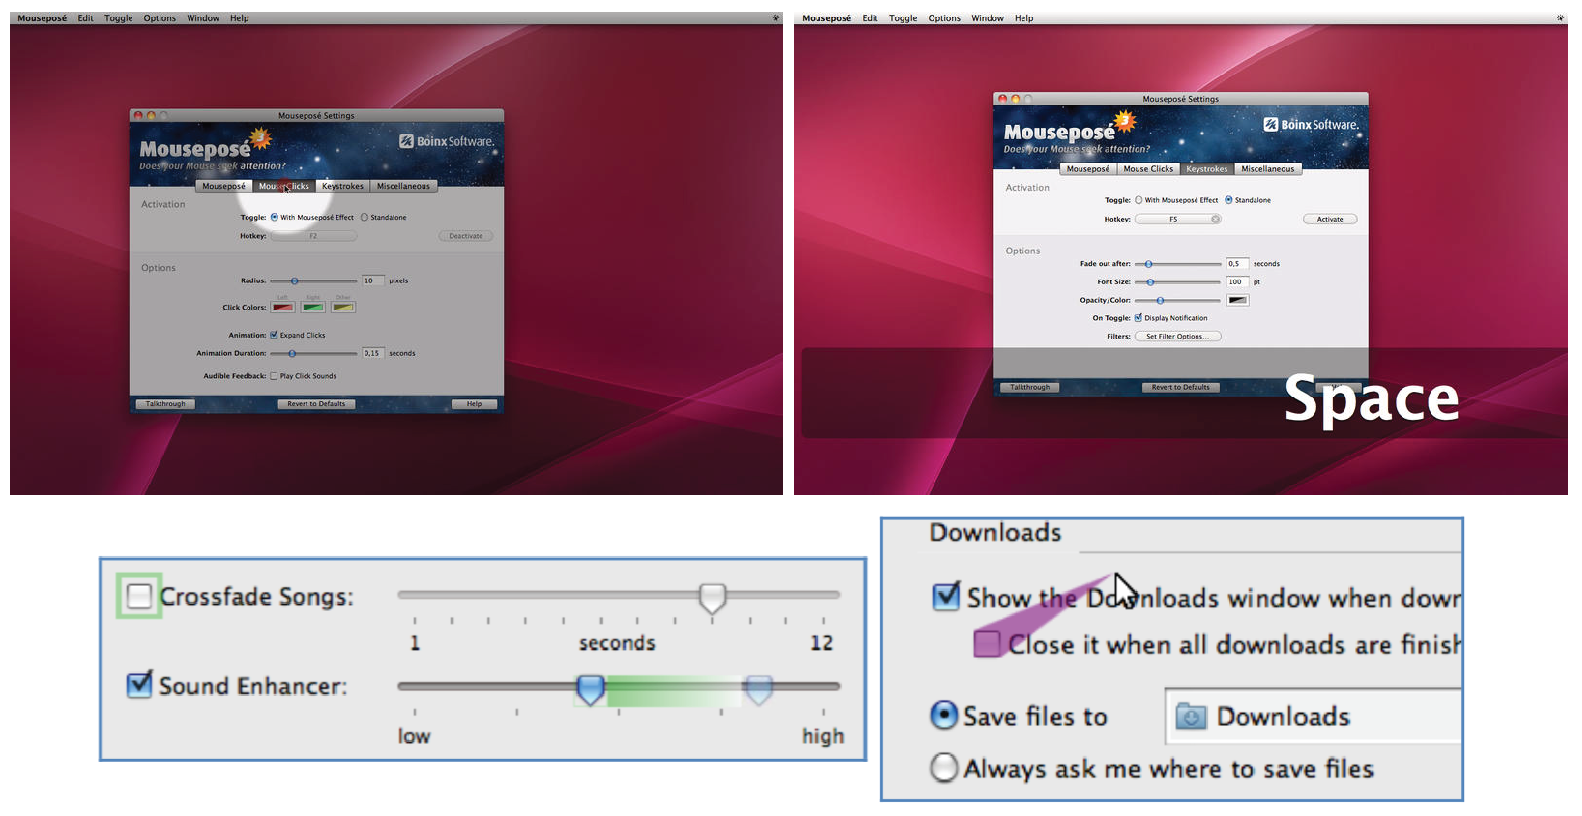
\includegraphics[width=0.7\textwidth]{\background/fig/realtime/realtime}
  \caption{Real-time visual enhancements on GUI applications: (top) Mouseposé highlights mouse cursors or text input; (bottom) Prefab creates target-aware or afterglow effects during user operating~\cite{Dixon:2010fb}.}
  \label{fig:related_realtime}
\end{figure*}

Real-time visual effects help users focus on the region of interest in a GUI application, but to support learners comprehend the application functionalities, there has been a considerable amount of research devoted to offering interactive helps.
%
Video snippets can be embedded in application tooltips~\cite{Grossman:2010wr}, which were shown to be seven times more effective than conventional tooltips for completing unfamiliar tasks.
%
Interactive, step-by-step instructions can be integrated in several forms:
%
To help user identify the correct UI components, tutorials can be shown via translucent colored ``stencils,'' which visually direct user's attention directly in an application~\cite{Kelleher:2005:STD:1054972.1055047}.
%
By tracking user's current operations, tutorials can be embedded in an application to provide instant feedback such as a check-mark or a percentage match~\cite{Fernquist:2011:SRE:2047196.2047245}, automatically replayed to provide the corresponding video instructions~\cite{Pongnumkul:2011ju}, or be shown as ambient help~\cite{Matejka:2011:AH:1978942.1979349}.
%
Instructions can be captured from demonstration as ``scripts'' for step-by-step navigation~\cite{Bergman:2005:DocWizards}. Having more user controls~\cite{Lieberman:2014:SML:2557500.2557543} or being enhanced with game elements~\cite{Li:2014:CGM:2556288.2556954, Dontcheva:2014:CCL:2556288.2557217} can further engage users in learning.

Last but not least, as tutorials are built for a broader community with a set of authors and learners, content can be dynamically updated within a community based on user contribution~\cite{Lafreniere:2013ff,Matejka:2009:CCR:1622176.1622214, Bunt:2014:TPI:2556288.2557118}.

interactive-visualization~\cite{Kwon:2016:CEO:2858036.2858101}
the paper that cited DemoWiz~\cite{Nguyen:2015:MST:2702123.2702209}

% These projects show how effective instructional representations can assist learners in learning or executing tasks. Our goal is to further study new formats that incorporate advantages of several formats of multimedia, including images, text, and videos, and in turn enhancing the learning experience for a variety of tasks.

% * define ``automatic''
% Note: MixT tutorials are automatically rendered from manual demonstration, not automatically generated.

% To provide real-time assistance, it is important to recognize the user activities during a task performance. Several domains have been widely studied, including software operations, scene recognition, and object tracking in a physical world.

% -------------------------------------------

\section{Instructions for Physical Activities}
\label{related_physical}

The above approach of tracking user behavior to automate tutorial authoring opens the door to interactive tutorials that can respond to user progress. However, tracking user behavior in the physical world, rather than in software, remains a challenge.

\subsection{Generating Instructions for Real-World Tasks}
Researchers have investigated tools for automatically generating visual instructions for physical tasks~\cite{feiner:1985:AEA:1299975.1300548,Seligmann:1991:AGI:127719.122732}. Workflows can be captured and created for furniture \cite{agrawala2003designing} or block assembly tasks \cite{Gupta:2012ku}.
%
If video content is difficult to be extracted, crowdsourcing algorithms have been introduced to structure step-by-step videos by online workers~\cite{Kim:2014:CSI:2611222.2556986}.
%
% New devices to support authors capturing multi-media materials, such as a turntable~\cite{Tseng:2015:SPT:2771839.2771869}
% documentation \cite{Tseng:2016:makeology}

\subsection{Interactive Guidance}
To provide responsive instructions, a computer system needs to understand user operations in real-time. Ideally, activities should be automatically tracked without human labeling.
%
Computer vision techniques can track specific physical targets, including hands \cite{Ranjan:2008}, user movements \cite{Wilson:2012fb}, fast-moving objects (e.g., a Ping-Pong ball) \cite{Okumura:2011tr}, or regions in pre-defined spaces \cite{Ranjan:2007}.
%
These methods usually require an expert defining heuristics of space regions or movement classifications ahead of time for the tracking program.
%
Thanks to the advance of technology, camera sensors such as Kinect have become widely available to track activities for block assembly~\cite{Gupta:2012ku} and dance~\cite{Anderson:2013:YEM:2501988.2502045}.

Real-time guidance is often shown via an external display, placed next to the working area~\cite{Gupta:2012ku}. To better blend the information into activities, Knibbe~\ea{} design a display-embedded table as a physical workspace that monitors, records, and assists users~\cite{Knibbe:2015:SMI:2817721.2817741}.
%
Alternatively, information can be overlaid on top of the work area using augmented reality, usually through a head-mounted display. Such systems can provide visual highlights for machine maintenance~\cite{Henderson:2011ff}, or interactive remote tutoring for repair tasks~\cite{Gurevich:2012ko}.
%
Another method is to overlay guidance on an augmented mirror for tasks such as dance movements~\cite{Anderson:2013:YEM:2501988.2502045}.

for Frisbee players~\cite{Solomon:2014:UTI:2540930.2540965}

% Lovell and Buechley use electrical sensing with conductive thread for a sewing tutorial~\cite{Lovell:2010tl}.

% I aim to propose a new approach that gives users flexibility in a home environment, and provides interactive control. If activity recognition is not possible, my approach includes users in the loop to annotate high-level information in order to create high-quality results.

% -------------------------------------------

\section{Working with Videos}

\tofix{intro here}

\subsection{Capture}
Several research and commercial systems guide users at capture time to yield higher-quality videos. Such systems often employ templates to help users capture sequences of distinct shots (e.g., Snapguide\footnote{\url{http://snapguide.com/}}) or suggest framing of the subject or camera view as in NudgeCam~\cite{Carter:2010}. Computer vision algorithms, like face tracking, can be used to offer real-time feedback during such directed actions~\cite{Davis:2003cu,Heer:2004ba,Carter:2010}. Instead of relying on templates, shot suggestions can also be bootstrapped through user dialogs~\cite{Adams:2005}.

\subsection{Annotation}
Researchers have investigated how to provide interactions that enable efficient, fluid annotation of video data, from the early EVA system~\cite{Mackay:1989} to more recent interfaces like VideoTater that leverage pen input~\cite{Diakopoulos:2006vt}.

\subsection{Editing}
Frame-based editing of video is very time-intensive, as it forces users to operate at a very low level of detail. Editors can leverage metadata, such as transcripts~\cite{Berthouzoz:2012,Pavel:2014:VDB:2642918.2647400} and shot boundaries~\cite{Casares:2002dx}, to give users higher-level editing operations at the shot level rather than the frame level.
In specific video domains like interview videos, transcripts can help users place cuts and transitions~\cite{Berthouzoz:2012}.
%
Computer vision techniques can automate certain effects, such as creating cinemagraphs~\cite{Bai:2012, Joshi:2012}, automatically-edited lecture videos~\cite{Heck:2007}, zoomable tapestries~\cite{Barnes:2010} and synopses~\cite{Pritch:2009vl}, or stabilizing shaky amateur videos~\cite{Liu:2011}. When analyzing video is a matter of subjective taste, identifying salient frames can also be outsourced to crowd workers~\cite{Bernstein:2011uj}.

live authoring through compositing and editing of streaming video~\cite{Freeman:2014:LLA:2611105.2557304}

\subsection{Navigating}
Videos can be navigated at the content level beyond log events, such as visualizing subject movements in a storyboard design \cite{goldman2006schematic} and enabling direct manipulation of a target in 2D \cite{Dragicevic:2008:VBD:1357054.1357096,Goldman:2008:VOA:1449715.1449719,Karrer:2008:DDM:1357054.1357097} or 3D \cite{Nguyen:2013:DMV:2470654.2466150}. These techniques help viewers understand content flow and playback videos, and have been applied to screencast videos \cite{Denoue:2013:RDM:2451176.2451190}. It is also possible to automate video control based on user actions for scenarios such as operating software applications~\cite{Pongnumkul:2011ju} and block assembling tasks \cite{Gupta:2012ku}. Such novel forms of video navigation inspired us to explore new visual designs for revealing the video content that support live presentations.

lecture videos~\cite{Tang:2006:DIU:1111449.1111523}

Visualization of personal history for video navigation~\cite{Al-Hajri:2014:VPH:2611105.2557106}

% In contrast to these systems, we do not require the author to manipulate the camera or system during capture. Many leisure activities, such as home repair or cooking, require use of both hands or involve getting one's hands dirty, so camera manipulation is not possible. We use vision techniques for automatic recording and editing. It differs from previous approaches in its focus on particular application domains -- software and physical demonstrations. By focusing on specific domains, we can make assumptions about the structure of the input and output video, such as the fact that there is a linear set of steps or movements, and offer user interfaces and algorithms that make it easier to create high quality instructions.

%!TEX root = ../thesis.tex
\section{Design Guidelines}

To motivate and inform the design of a tool to support live presentations, we collected preferences for software demonstrations using an online survey. We describe the three design goals derived from the survey results.

\subsection{Understanding Demo Preferences} To understand both presenters' and audiences' preferences for performing and viewing system demonstrations, we conducted an online survey in a software company and a university research lab. Our goal was to collect people's feedback on giving and seeing software demonstrations during live presentations. We received 73 responses from researchers, graduate students, software engineers, and designers. Their main research areas include human-computer interaction (64.4\%), software engineering (21.9\%), and machine learning (20.6\%); 66.7\% were male. Among all the respondents, 35.6\% indicated that they were very experienced at giving software demos to the audience during a live presentation; 46.6\% had demoed at least once; 13.7\% had not demoed but attended talks that showed a software demonstration.

We asked respondents who had demo experience (\textit{N} = 60) how they preferred to perform a demo. Their answers were: a live demo (25 out of 60), pre-recorded videos (15), a mixed format of a live demo and videos (12), static screenshots (4), and other (4). In Table~\ref{tab:demowiz_survey}, we list the top 2-3 reasons for their preferences. Giving a \textit{live demo} can be more engaging with a working system and match the audience's interests, but presenters can encounter unexpected problems and forget to show important features within a given time constraint. On the other hand, presenting with \textit{a demo video} avoids such problems by extracting the most important parts, and can allow visual highlighting (labeling or zooming), but can be less engaging. In addition, it is hard to narrate.

We were also interested in reactions as an audience member. For respondents who had seen software demos (\textit{N} = 70), we asked how they preferred to see the demonstration performed. We found a slightly different preference: a live demo (36 out of 70), a mixed format of a live demo and videos (24), pre-recorded videos (7), and other (3). However, the reasons were well aligned with presenters’ concerns. A\textit{ live demo} shows a working system and can be more engaging, but the audience might need to wait for system problems to be resolved or sometimes see presenters rambling. A\textit{ demo video }can show the most important parts, sometimes assisted by visual highlighting, but it can be hard to tell which parts of a demo are real, and can be less engaging to the audience.

\subsection{Design Goals} From the survey results, we understand that giving a live demo is often more preferable than showing demo videos. However, we cannot, in general, address some of the main concerns with giving a live demo – that is, stability of the software system and variations in the presentation environment which can cause the demo to fail. Therefore, we instead aim to address some of the drawbacks with demo videos while preserving their advantages. More specifically, our goal is to make demo videos \textit{more engaging} by assisting presenters in adjusting their narration to guide the audience through the material. In this section, we describe our design goals to support more effective demo video presentations.

\subsubsection{G1. Show what's coming next, where and when it will occur.}
To engage the audience with the demonstration, it is important for presenters to guide the audience's attention to the right place at the right time. To do so, presenters should be fully aware of upcoming actions – specifically \textit{what} actions will happen, \textit{where} they will occur on the screen, and \textit{when} they will happen.

\subsubsection{G2. Minimize required attention or interpretation.}
While it is our desire to help presenters understand and anticipate impending events, we should not overburden a presenter who is already narrating a specific set of talking points. As a tradeoff between providing more information and minimizing cognitive load, any augmentation of the video needs to be offered in a glanceable fashion, i.e., information can be interpreted quickly and without the presenter's full attention.

\subsubsection{G3. Support light-weight editing during rehearsal.}
Different presentations may require more or less extensive explanations, and when first recording a demo video, it may not be possible to perform the demo at the same rate necessary for a live presentation (e.g., typing can be difficult or system response times may be variable). In addition, it should be easy to review, practice, and modify the pace for a particular presentation. For all these reasons, lightweight editing and rehearsal are necessary.  Using these principles as a guiding rubric for our design, we iterated on several versions of the DemoWiz system.

\begin{table}
  \centering
  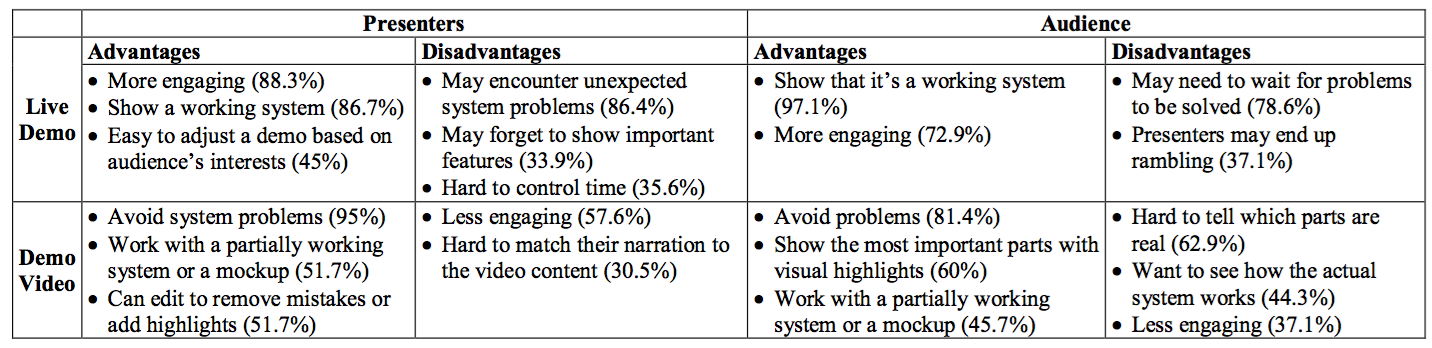
\includegraphics[width=\columnwidth]{\demowiz/fig/survey}
  \caption{Survey of software demonstration preferences from presenters' (N=60) and audience's (N=70) point of views.}
  \label{tab:demowiz_survey}
\end{table}

%!TEX root = ../thesis.tex
\section{Computer-Generated Visualization}

\subsection{Augmented Workflow}
For presenters to narrate ``live'' over a video recording, we propose augmenting a typical workflow from capturing a screencast video; to rehearsing it and adjusting timings; and finally to live presentation of the demo video (Figure~\ref{fig:demowiz_workflow}).

DemoWiz first captures a screencast video and input events during a software demonstration from a user-defined rectangular region. Once the recording is done, DemoWiz analyzes the low-level event stream and transforms it into higher-level events such as mouse clicks, double-clicks, and drags. DemoWiz then allows presenters to edit the timing and notes while practicing their presentations with the presenter view equipped with an adjustable event timeline (Figure~\ref{fig:demowiz_teaser}A). Finally, presenters can give a live presentation using the same UI (i.e., presenter view) and show the audience view without visualization to the viewers.

\begin{figure*}[t]
  \centering
  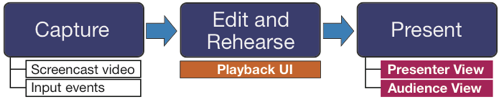
\includegraphics[width=0.7\textwidth]{\demowiz/fig/demowiz_workflow}
  \caption{DemoWiz workflow: Presenters captures a software demonstration, edit the video recording while rehearsing with our playback UI, and present the edited video to the audience using a presenter view.}
  \label{fig:demowiz_workflow}
\end{figure*}

% ---------------------------------------------------------------

\subsection{Visualizations}
To enable presenters to focus on their narration and the original video contents, DemoWiz augments the screencast recording by automatically overlaying simple glyphs.

\subsubsection{Input Event Glyphs}
DemoWiz overlays visual annotations of events on the screencast recording in a graphical way where the events happen.For example, in Figure~\ref{fig:demowiz_teaser}, the presenter clicks and drags the map view to the right. DemoWiz uses the following simple,distinctive glyphs to differentiate event types as Figure~\ref{fig:demowiz_glyphs} shows:

\begin{itemize}
  \item Mouse click: a red circle with a radius of 20-pixels,
  \item Double-click: a green circle with a radius of 20-pixels,
  \item Mouse drag: a thin, orange line with a dot at the start point and an arrowhead at the end point,
  \item Mouse scroll: a thin, yellow line, 80 pixels long, with an arrowhead, and
  \item Keystrokes: text in blue.
\end{itemize}

At any given time during the video playback, DemoWiz shows the current event and the upcoming event on the video. We tried to show more than two events within a fixed time period in our initial prototypes. However, we noticed several issues. First, the view becomes too cluttered to understand at a glance, especially when the original video is visually complex. Second, it is not easy to convey the order of the events. Third, it is difficult to observe when multiple events are spatially close. Therefore, we provide minimum but essential events for recall.

\begin{figure*}[t]
  \centering
  
\includegraphics[width=0.7\textwidth]{\demowiz/fig/event_types/types}
  \caption{DemoWiz visualizes input events in a graphical way. From the left to right we show a mouse click, double-click, a drag, a mouse scroll, and keystroke events. These glyphs are overlaid on the video recordings.}
  \label{fig:demowiz_glyphs}
\end{figure*}

% --------------------------------------------------

\subsubsection{Visual Guides to the Next Events}
In order to help guide the presenter's attention, DemoWiz overlays a motion arrow between the current and upcoming events on the demo video (Figure~\ref{fig:demowiz_teaser}C). This is inspired by storyboard design used in filming where an arrow effectively shows the movement of a camera or an actor in a single shot \cite{goldman2006schematic}. We expand the idea of guiding attention for a specific purpose: the arrow in DemoWiz shows the movement from one action (e.g., click a checkbox) to another action(e.g., click a button). By overlaying this motion arrow, the visualization matches the flow of a presenter's attention when they observe the video content.

Since the distance between two consecutive event segments vary, we created three visual designs to make sure the arrows are visible to lead a presenter's attention:

\begin{itemize}
  \item For two events that are located far away (e.g., clicking an ``OK'' button after selecting a checkbox on a page), apply a \textit{straight} arrow (see Figure~\ref{fig:demowiz_arrows}A).
  \item For events that are nearly at the same location (e.g., click the ``Next'' button twice to navigate a list of selections),apply a \textit{round} arrow that points to the current location (see Figure~\ref{fig:demowiz_arrows}B).
  \item Otherwise, apply a \textit{curved} arrow (see Figure~\ref{fig:demowiz_arrows}C).
\end{itemize}

\begin{figure*}[t]
  \centering
  \includegraphics[width=0.6\textwidth]{\demowiz/fig/arrows/arrows}
  \caption{Three types of motion arrows in DemoWiz that guide presenters to the next event of different distances at a (A) far, (B) nearly the same, and (C) near location.}
  \label{fig:demowiz_arrows}
\end{figure*}

% --------------------------------------------------

\subsubsection{Sense of Timing}
DemoWiz provides a sense of timing for an upcoming action so that presenters can adjust their narration. First, DemoWizembeds \textit{a progress bar} in the motion arrow to show relative time (Figure~\ref{fig:demowiz_teaser}C). The green bar shows the proportional time that has been passed before reaching the next event (Figure~\ref{fig:demowiz_timing} top). When a motion arrow is filled up with green, it fades away and guides the presenter to the next action. We were concerned that people may associate the length of an arrow to the length of time. Therefore, we also incorporated a \textit{countdown} visualization where circles will fade out in the last three seconds before the next action starts (Figure~\ref{fig:demowiz_timing} bottom) to convey absolute timing.

\begin{figure*}[t]
  \centering
  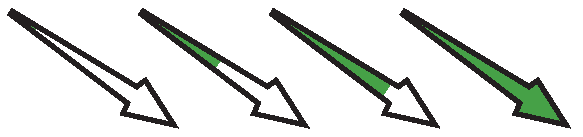
\includegraphics[width=0.6\textwidth]{\demowiz/fig/progressbar/progressbar}
  
\includegraphics[width=0.6\textwidth]{\demowiz/fig/countdown/countdown}
  \caption{A progress in time guides the presenter from the current event (left) gradually to the upcoming action (right) using relative timing with a progress bar (top) and absolute timing (bottom).}
  \label{fig:demowiz_timing}
\end{figure*}

% --------------------------------------------------

\subsubsection{Visualization Examples}
Figure~\ref{fig:demowiz_examples} presents examples of DemoWiz visualizations with four different systems. The glyphs effectively show the start and end points of mouse drags and the locations of mouse clicks. Motion arrows help direct the presenter's attention between events, such as start the end of the drag event to clicking a button (Figure~\ref{fig:demowiz_examples}A and B), clicking between several options (Figure~\ref{fig:demowiz_examples}C), or selecting a specific slide after scrolling down (Figure~\ref{fig:demowiz_examples}D).

\begin{figure*}[t]
  \centering
  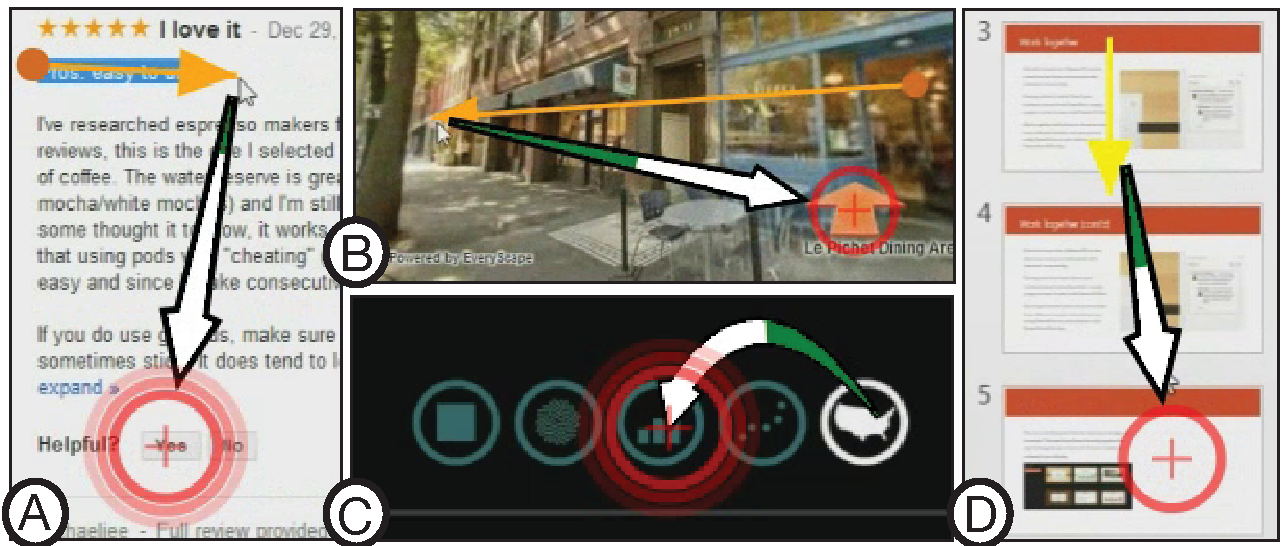
\includegraphics[width=0.7\textwidth]{\demowiz/fig/examples/examples}
  \caption{Examples of DemoWiz visualizations with four different systems and input event sequences.}
  \label{fig:demowiz_examples}
\end{figure*}

% ---------------------------------------------------------------

\subsection{Lightweight Editing During Rehearsal}
During rehearsal for their demonstration, presenters can modify the video timing and add reminder notes for their narration. DemoWiz shows the type and length of each event in a sequence in a timeline (Figure~\ref{fig:demowiz_teaser}A). Each segment is shown as a block whose width indicates its length in time. To simplify the timeline and avoid fine-grained adjustment,lengths of event blocks are rounded to the second. Presenters can modify the playback speed of a segment by dragging the boundaries of a segment on the timeline. For example, presenters can speed up to shorten long text inputs, and slowdown for fast mouse drag inputs that select multiple objects.

Sometimes a change in the playback speed may result in an awkward effect that is noticeable to the audience, especially when showing a UI transition. Therefore, DemoWiz supports two special time control markers to enable breaks in the narration. Presenters can add an adjustable \textit{pause} segment, at which the system will pause at the last frame of the previous segment for the specified length of time. If presenters prefer full control on pause length, a \textit{stop} marker ensures the video stays paused at the last frame of the previous segment and will not proceed until presenters manually resume the playback of the video.DemoWiz enables presenters to add a short text note (such as the reminder \iquote{Move and zoom...} in Figure~\ref{fig:demowiz_teaser}) so that they could remind themselves of upcoming actions at a higher level. The note can be positioned manually at any location on a video so that it does not block important video content, and will be shown for 3 seconds before the associated event.For every edit that is associated with time changes (including playback speed and pauses), DemoWiz computes and updates the total presentation time as well as updating the progress bar and countdown to provide accurate timing.

% ---------------------------------------------------------------

\subsection{Presenter View}
During presentation, DemoWiz shows two views in separate windows. Presenters can observe visualizations using the presenter view, while the audience will see the audience view with a full-screen video that has no enhanced information. DemoWiz synchronizes the videos in both views based on presenters' editing decisions to ensure the same playback speed and time. As with a conventional video player, presenters can control the video, to pause and play at any time. In addition, when a video is paused (or stopped), presenters can hover the mouse over the demo video in the presenter view to point out an important area, as many presenters currently do in a live demo. DemoWiz then simulates and synchronizes a mouse cursor in the audience view to help the audience follow the demonstration.

% ---------------------------------------------------------------

\subsection{Implementation Details}
During recording, DemoWiz captures the screen within a specified region and logs low-level system input data with\textit{timestamps} (with an accuracy of 0.1 seconds) from the operating system, including:

\begin{itemize}
  \item \textit{Mouse events} (mouse downs, mouse ups, and mouse wheel movements) and their \textit{positions} (in x-y coordinates relative to the screen-captured region).
  \item \textit{Key-press events} (keyboard input).
\end{itemize}

Once presenters finish their demonstrations, DemoWiz analyzes the low-level event stream and transforms it into high-level event metadata. For mouse events, we pair each mouse down and up into mouse \textit{clicks}, \textit{double-clicks}, or \textit{drags}. We group any consecutive mouse wheel events within a time threshold of 2 seconds to one \textit{scroll} event and any key-press events within the same threshold to one \textit{keystroke} event(e.g., combine keys d-o-w-n-t-o-w-n to ``downtown''). For each high-level event, we log the \textit{start} and \textit{end time} (timestamps of the first and the last low-level event).

Based on the start and end times of these high-level events, DemoWiz segments the screencast video recording into \textit{event segments}. Any gap between two consecutive input events is marked as an \textit{inactive segment}, which may include mouse hovering, UI transitions of the demo system, or static frames with no visual changes. DemoWiz adjusts the boundaries of these event segments to avoid any short visual effect that cannot be observed. DemoWiz examines segments in a linear order to ensure each segment lasts at least $t_{min}$ seconds long,which is set as one second based on our early testing. For an event segment $S_i$ of time ($t_{start}$, $t_{end}$) that $t_{end} - t_{start} < t_{min}$, DemoWiz expands 0.5 second forward and backward if $S_{i-1}$ and $S_{i+1}$ are inactive. If the adjusted $S_{i-1}'$ and $S_{i+1}'$ are shorter than $t_{min}$, DemoWiz merges it to the shorter neighbor segment. Currently, DemoWiz does not analyze these inactive segments, but techniques including computer vision and video analysis \cite{Banovic:2012kd,Chi:2012:MAG:2380116.2380130} can be applied for finer segmentation.

The capturing program is implemented in C\#. Two APIs were used: 1) the Windows Event Log API for mouse and keyboard hooks and 2) the Expression Encoder 4 API for screen recording running on Microsoft Windows 7. The recorded metadata(stored in a JSON object) and screencast video (in MP4) are read by the Presenter UI, which is implemented using standard Web technologies, including HTML5, CSS3, JavaScript, and jQuery. In particular, the visualization is rendered on the canvas element on top of the video object on the fly based on the video playback time. The audience view is generated by the main browser window of presenter view for video control.

%!TEX root = ../thesis.tex
\section{Evaluation}
To evaluate the DemoWiz design, we conducted a controlled experiment in which participants recorded and edited a demo video, and gave a presentation with the edited video. Specifically, we wanted to see if presenters would evaluate their own performances higher with the support of our augmented visualizations and control of timing.

\subsection{User Study}

\subsubsection{Baseline Condition: DemoWiz without Visualization}
Since DemoWiz allows for rapid editing of the video, it would have been unfair to compare it with a conventional video player without supporting any editing during the rehearsal phase. We therefore modified our system to serve as the baseline condition, providing participants with the same lightweight editing of the video in each condition. However, during presentation, the baseline condition was similar to a conventional video player that shows only the video without event timeline and augmented visualizations. It also did not support the \textit{stop} markers and \textit{text notes}, i.e., participants could only adjust playback speed of each segment and add variable length \textit{pauses}. During presentation, participants only saw the video with a traditional timeline. They could, however, pause (or stop) and resume the video manually at any time during playback.

\subsubsection{Study Design}
We conducted the study as a within-subjects design in a usability room. After recording and editing a video using the same system, each presenter gave a presentation with both systems to an experimenter. To control the effect of order and learning, we prepared two tasks that included similar interaction flows and counterbalanced the order of the two systems—DemoWiz and Baseline—-but we fixed the order of tasks. Even though presenting to a single audience member in a usability room is not the same as using the system with a large conference audience, it is important to control the tasks and presentation as closely as possible to understand the relative benefits of the system in comparison with a baseline condition.

For each condition, we observed and coded the \textit{timing} of narration that matched the video content and noted the time in seconds when an event was described \textit{before}, \textit{at}, or \textit{after} the action happened in the demo video. We also marked obvious \textit{breaks} between narrations, \textit{errors} when the narration was not about the current or following events (e.g., discussing actions in a different order than they actually occurred), and \textit{misses} when an important action was not mentioned. To avoid unconscious bias that might influence the coding of the videos, we neutrally named the recordings and coded them all in a batch. We focused on objective timing measurements as much as possible, measuring deviation from specific video events and their corresponding narrations down to a second. Finally, we gathered qualitative feedback through satisfaction and preference questionnaires.

\subsubsection{Participants}
We recruited 12 participants (10 males and 2 females) from a software company. However, we excluded the data from two participants (1 male and 1 female); one was due to a software bug during one condition and another was because the participant requested to restart a presentation in one condition. The average age of the effective 10 participants was 37.3 ranging from 24 to 64 years of age. We recruited participants who had experience at showing a software demonstration to an audience such as giving a presentation at a conference. Four participants were native English speakers and the rest were fluent in English. The expertise of participants included audio processing, computer graphics, human-computer interactions, machine learning, networking, and software engineering. Each participant was compensated with lunch coupons worth \$20.

\subsubsection{Procedure and Tasks} Each session consisted of one training task and two experimental tasks. For the training task, to introduce the common features for recording and editing the video, we designed a simple workflow of five steps to demonstrate editing of a slide using PowerPoint. The experimenter briefly demonstrated an example and then introduced the recording program that captured the screen. Participants were then asked to practice and record using the recording program.

The two tasks consisted of a similar sequence and interactions: 1) searching with Bing Maps to show the 2D map view and the Bird's Eye view, looking for a restaurant, and navigating to the interior view of a specific restaurant; and 2) searching with Google Shopping to show the search results with the Grid view, filtering and voting for reviews, and navigating the 3D product view of an espresso machine. For each task, we provided a specific scenario along with a list of subtasks. The experimenter walked through this list with participants to ensure that they could easily find the features that needed to be demonstrated. Participants were then asked to practice (3-5 minutes), record (about 2 minutes), and rehearse and edit (5-10 minutes).

To help simulate a conference setting where participants would not be able to present immediately after having recorded a demonstration, we inserted an intentional 1-minute gap between rehearsal and presentation. During this gap before giving the presentation, we asked participants to watch a conference showcase video. Participants were then asked to stand up and gave a 2-3 minute presentation to the experimenter in a usability room.

After each task, participants filled out a questionnaire of 8-10 questions asking about their experience (8 for the Baseline condition, and 10 for the DemoWiz condition). At the end of the session, an online questionnaire was provided for them to present overall preferences and leave comments. Each session lasted about 1.5 hours.

\subsubsection{Experiment Setup}
Each participant used a desktop computer running Windows 7, Expression Encoder 4 for screen recording, and a web browser for the DemoWiz user interface. A regular mouse and keyboard were provided, along with two 27-inch displays, one for editing (during rehearsal) and showing the audience view (during presentation), and the other for the presenter view on a stand-up table. The resolution of both displays was 1920×1200 pixels. The average captured screen area was 1311×857 pixels. In the presenter view, the video resolution was within 1000×600 pixels; in the audience view, the screencast videos were resized to fill the entire display with at least 100-pixel wide border in black. During the study, the experimenter stayed in the room, providing instructions and sitting behind the participants during the recording and editing phases.

% ---------------------------------------------------------------

\subsection{Results}
Ten participants successfully recorded, rehearsed, and gave a demo with both systems.

\subsubsection{Subjective Preference}
Figure~\ref{fig:demowiz_likert} shows the average subject responses (on the 7-point Likert scale) from presenters for both systems. We analyzed these subjective responses using a Wilcoxon signed-rank test. We found significant differences in responses for ease of narration (DemoWiz µ = 6.2 over Baseline µ = 4.5, \textit{p} = .018) and ease of presentation (6.4 over 5.2, \textit{p} = .048). We also found marginally significant differences in participants' overall satisfaction with their presentations (5.5 over 4.7, \textit{p} = .062). Participants also tend to agree that DemoWiz helped them interpret timing (6.1 over 4.4, \textit{p} = .067).

In addition, 9 out of the 10 participants preferred DemoWiz to the system without visualization and would choose to present with DemoWiz if they were asked to give a public software demo; the remaining participant indicated no preference for both questions. The general feedback was also encouraging. For example, P1 commented \iquote{Awesome system. I'd use it today.} and P5 \iquote{felt more confident in being able to present what I wanted to.}

\begin{figure*}[t]
  \centering
  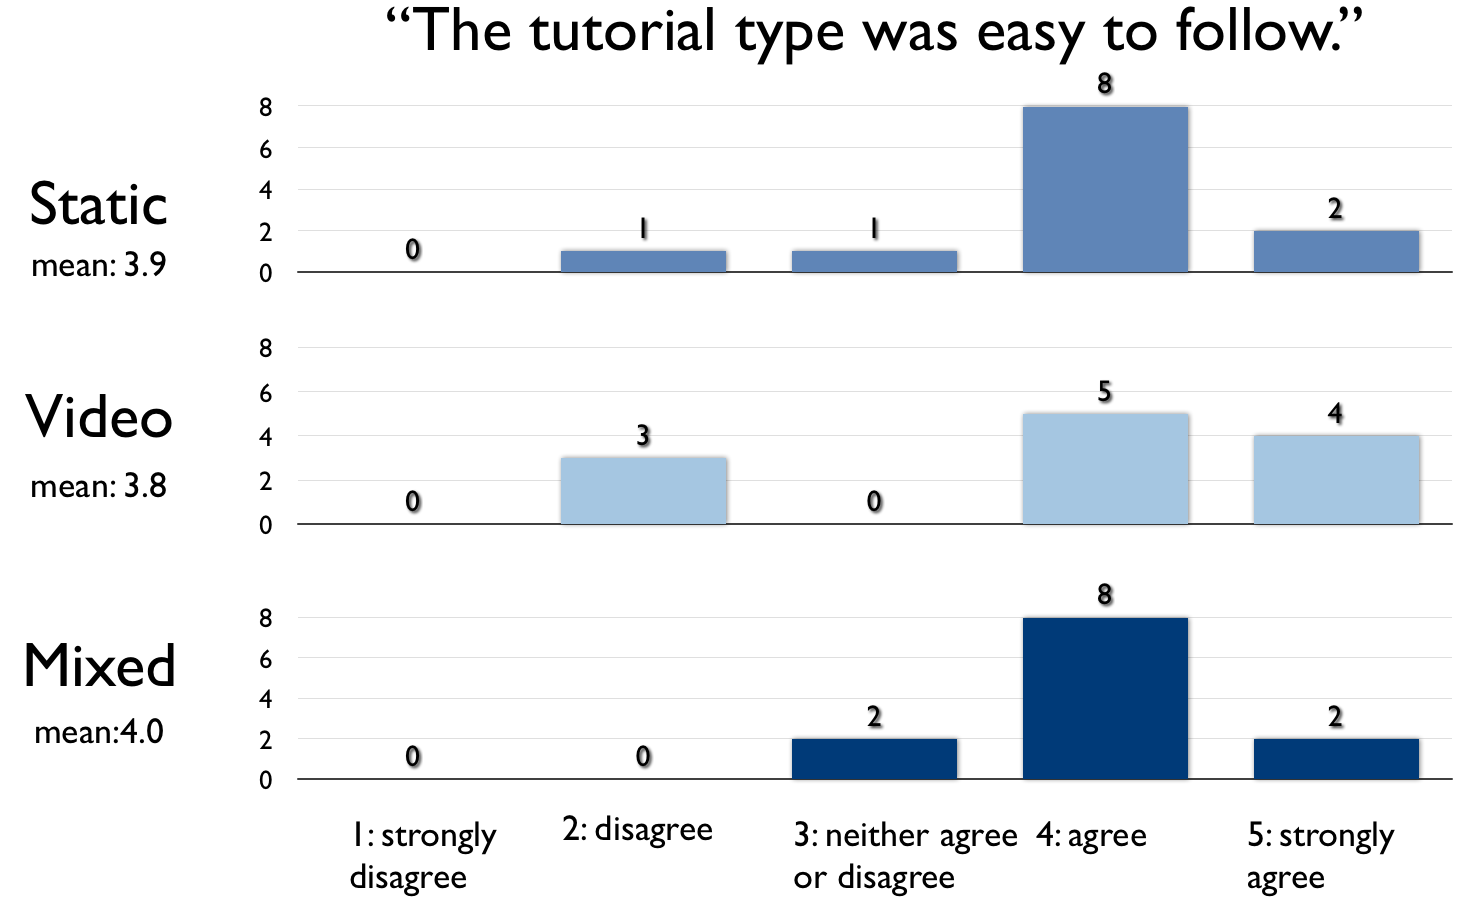
\includegraphics[width=\textwidth]{\demowiz/fig/results/likert}
  \caption{User feedback from questionnaire on the 7-point Likert scale.}
  \label{fig:demowiz_likert}
\end{figure*}

\subsubsection{Visualization as a Supportive Cue}
Participants answered that they were able to understand DemoWiz visualization of input events (µ = 6.0) and found it supportive for their presentations (µ = 6.3). They also commented that the DemoWiz visualization supported the presentation in various aspects: \iquote{the visualization reminds of the order of the content} (P1), \iquote{Really liked the ability to know what was coming up} (P2), \iquote{It provides better insight of the progress of the video} (P6), and \iquote{viz gave me an idea about timing or something I was going to forget to say} (P9).

\subsubsection{Narration Timing}
We coded the 20 recordings of participants' final presentations to observe the timing of narration of each action in correspondence with the video content (11 key events for both tasks). With DemoWiz, participants tended to \textit{anticipate} the upcoming events rather than talk afterwards, where the average timing was -0.1 seconds with DemoWiz (i.e., narrated the action before it happened) and 0.4 seconds with the Baseline condition (i.e., explained the action after it was shown). We found a significant difference in the number of times that events were anticipated by the narration, co-occurred, or occurred after the fact ($\chi $\textsuperscript{2}\textit{(2,220) = 8.6, p = .01}, see Figure~\ref{fig:demowiz_results_timing}).

In general, this supports our suspicion that DemoWiz would help in anticipating an event as opposed to talking about it after it occurred. More important though, was how often a narrator spoke about an event within several seconds of when the event actually occurred. By defining \textit{better} timing as when a presenter's explanation came within 2 seconds of a shown event (either prior, exact, or after), there was marginal significance by condition (\textit{p} = .089 with DemoWiz performing better). In addition, with the Baseline condition, the timing of narration was less consistent and off more, varying from 6 seconds early or 10 seconds late with a variance of 3.9 seconds, in comparison to the DemoWiz condition with at most 3 seconds early to 3 seconds late and a variance of 1.9 seconds.

Five participants had an obvious \textit{error} (forgot the next action or incorrectly narrated another action), had a long \textit{break} (waiting for more than 2 seconds until the action was made), or \textit{missed} an action (did not explain an important feature) when presenting with the Baseline condition. On the other hand, in the DemoWiz condition no errors were made, and there were only one long break and one miss from two different participants, respectively.

Participants' comments also support the fact that DemoWiz helped presenters anticipate the upcoming events. P7 explained, \iquote{(I) felt better able to time my speech to coincide with visual events, rather than trailing after them. Without the event visualizations, I felt like I was talking about what the audience had just seen, rather than having my words and visuals combine to a single message.}

\begin{figure*}[t]
  \centering
  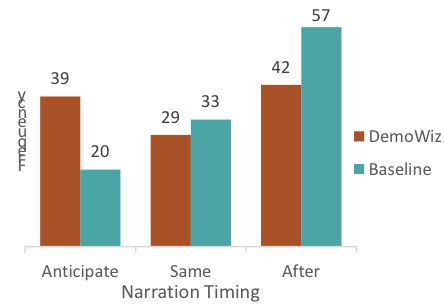
\includegraphics[width=\textwidth]{\demowiz/fig/results_timing}
  \caption{The number of times events were anticipated by the narration, co-occurred, or occurred after the fact.}
  \label{fig:demowiz_results_timing}
\end{figure*}

\subsubsection{Editing Experience}
We collected comments on the workflow. Participants found it easy to record (µ = 6.4) their demonstrations with DemoWiz. For editing features, they found it easy to edit in general (6.6), including controlling the playback speed (6.5) and adding pauses and stops (6.5), but it was less easy to add text notes (4.8); only two participants used this as reminders.

Although using different strategies, all of the participants adjusted the playback speed for matching their narration. Some sped up whenever possible and added stop markers for transitions; some slowed down the repetitive actions (such as drags) to demonstrate effects. P6 said, \iquote{I really liked being able to add ‘stop' events so I could \'fake\' my demo better.} DemoWiz made it easy for participants to separate the capturing and presentation preparation as P5 explained, \iquote{Overall, recording was very easy. In fact, as I got to the second task, I realized that I really don't need to think about the words as I record because later on I will be able to slow down and speed up time ...}

On average, the length of demo videos was 2'09\" before editing and 2'05\" after editing, and the presentation was 2'38\" long. Each participant spent 7.5 minutes on average to edit. For each demo of 44 segments on average, participants adjusted 3.15 segments for speedup and 4.25 segments for slowdown, and added 0.55 pause markers. In the DemoWiz condition, 1.2 stop markers and 0.2 text notes were added.

%!TEX root = ../thesis.tex

\subsection {Discussion}

%We discuss general findings from the 3 studies.
% \dan{Make this a discussion about all 3 studies together, what was learned overall? Argue that DemoDraw is good.}
%
Participants were clearly excited about the overall experience using both the \phaseI{} and the \phaseII{}.
%Comments we received included, \systemname{} is a \iquote{REALLY COOL SYSTEM} (Study 2-P7), \iquote{Seriously, the poses look really cool! I want the last one to be my profile picture} (Study 2-P3), and \iquote{Great idea overall, this will save lots of time for whoever is designing these artworks :)} (Study 3-P3).
%
Some explicitly pointed out their enjoyment when using our system:
% \iquote{Overall, it's a lot of fun, and I can see it being really helpful for anybody trying to explain motion} (P3),
\iquote{it accurately captures how much fun I had making it. :)} (Study 2-P9), and
\iquote{For professional artists, the system not only increases their productivity, but also brings joy and fun to this kind of tasks} (Study 2-P10).

Participant feedback suggests motion illustrations generated by \systemname{} are expressive enough to depict their demonstrations. Our multi-modal interface with our motion analysis and rendering algorithms enabled users to quickly create step-by-step diagrams. Recall that current methods using existing software tools to create similar diagrams take significant time and making visual or spatial changes is difficult.

\bjoern{I'm not really sold on the rest of this section - some of it feels too low level. Not sure what to do here.}

\dan{One of the main things to discuss (with some convincing arguments based on specific results from the three studies) is whether we achieved our primary goals and answered research questions:
1) the system makes good looking diagrams quickly; (reference back to how long current methods take)
2) the iterative/interactive demonstration style is key to this success. (reference back to how non-iterative current methods are) }

\dan{Another discussion topic is the implications of this system. If the iterative/interactive demonstration style worked here, would it be better in other demonstration systems too? What should interaction designers learn from this at a level above the specific motion illustration task?}

\subsubsection{Illustration Styles}
In Study 1, motion arrows successfully conveyed the majority of movements. For some movements when arrows failed to express the intent, other illustration effects might clarify the details to depict the start, intermediate, and end poses. For example, in the first motion set of Study 1, the circular hand movements and squatting action of Step 3 might not be easily interpreted (see Table~\ref{tab:study1_errors}), but for the same motion, participants preferred stroboscopic effect that clearly showed the arm movements and transition in height (see Figure~\ref{fig:study3_effects}).

Furthermore, as \systemname{} captures the continuous motion sequence in 3D from a demonstrator, our system also generates animations showing the dynamic movements.
%
In the warm-up task of Study 2 that captured the second motion set in Study 1, some participants explained that the playback animation of the recording clarified the motion where they incorrectly interpreted the start position.
%
We propose that as motion arrows can efficiently and effectively express most of the motions, a mixed-media version can be created that has been shown to be useful for clarifying step-by-step instructions \cite{Chi:2012:MAG:2380116.2380130}, where viewers can selectively review part of a static diagram with in-place animation playback. In addition, the 3D reconstruction also makes it possible to review motions from different angles.
%
All in all, our technology enables both instructors and viewers to interactively create and review motion illustrations in multiple ways.

%!TEX root = ../thesis.tex
\chapter{Discussion}
\label{chapter_conclusion}

\section{Restatement of Contributions}
In this dissertation,

% How to design tutorial systems appropriately for different situations
% * level of expertise of instructor, learner
% * what are you trying to make easier?

\section{Remaining Challenges and Future Directions}

formal language
- now template, a set of techniques

\subsection{Collaborative Authoring}
a team, beyond a single author for larger projects or tasks

\subsection{Non-Linear Tutorials}
branching

\subsection{Mobile Capturing devices}
Tango, Structure Sensor, Leap Motion

\subsection{Emerging Instructional Space}

Augmented and virtual reality systems are becoming available to end users via affordable forms. However, designing AR and VR experiences extremely requires expertise and efforts. As devices offer personalized effects supported by sensing and input techniques, we need new authoring tools that focus on delivering story-centric experiences. Tools should also enable both professionals and amateurs to create and iterate designs efficiently in an immersive 3D world. ...research what future AR and VR creation tools would look like with new authoring processes.

by demonstration
``Microsoft HoloLens with Autodesk MotionBuilder'' by Jasper Brekelmans, \url{https://www.youtube.com/watch?v=yfl7pwXftUs}, licensed under CC BY 2.0


\begin{figure*}[ht!]
  \centering
\begin{tabular}{cc}
  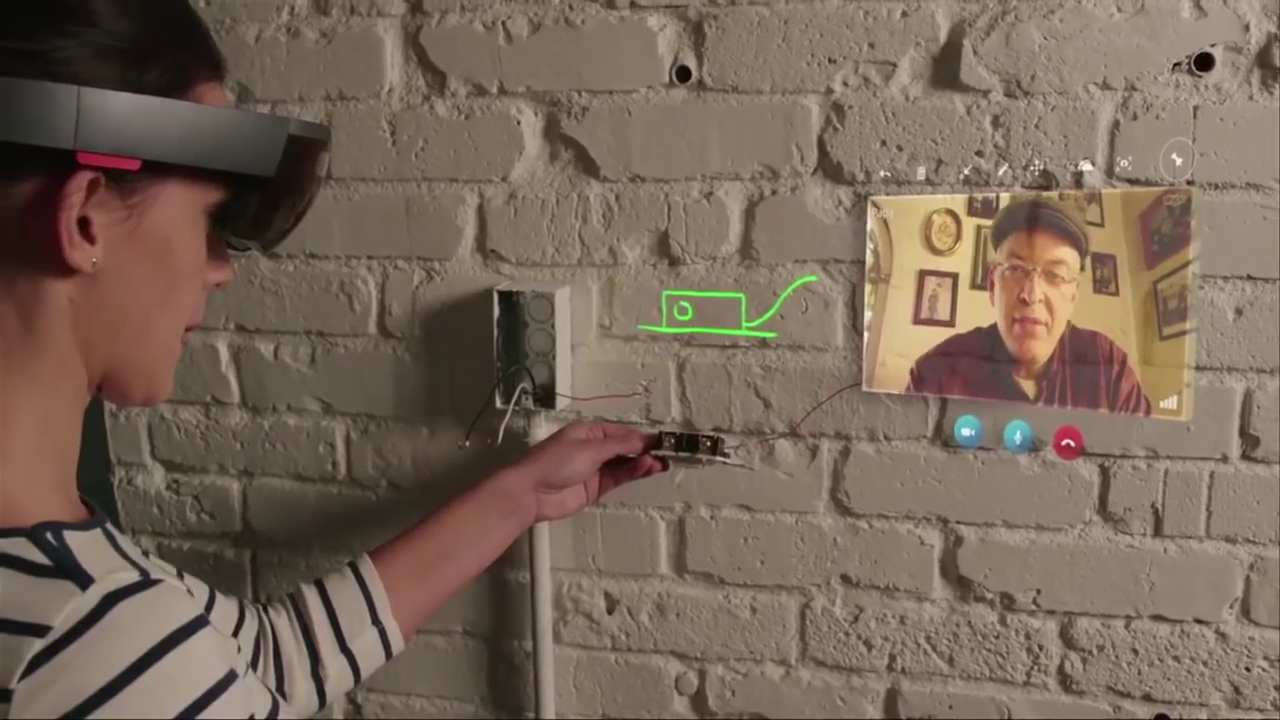
\includegraphics[width=0.4\textwidth]{\conclusion/fig/ar/hololens_fix1} &
  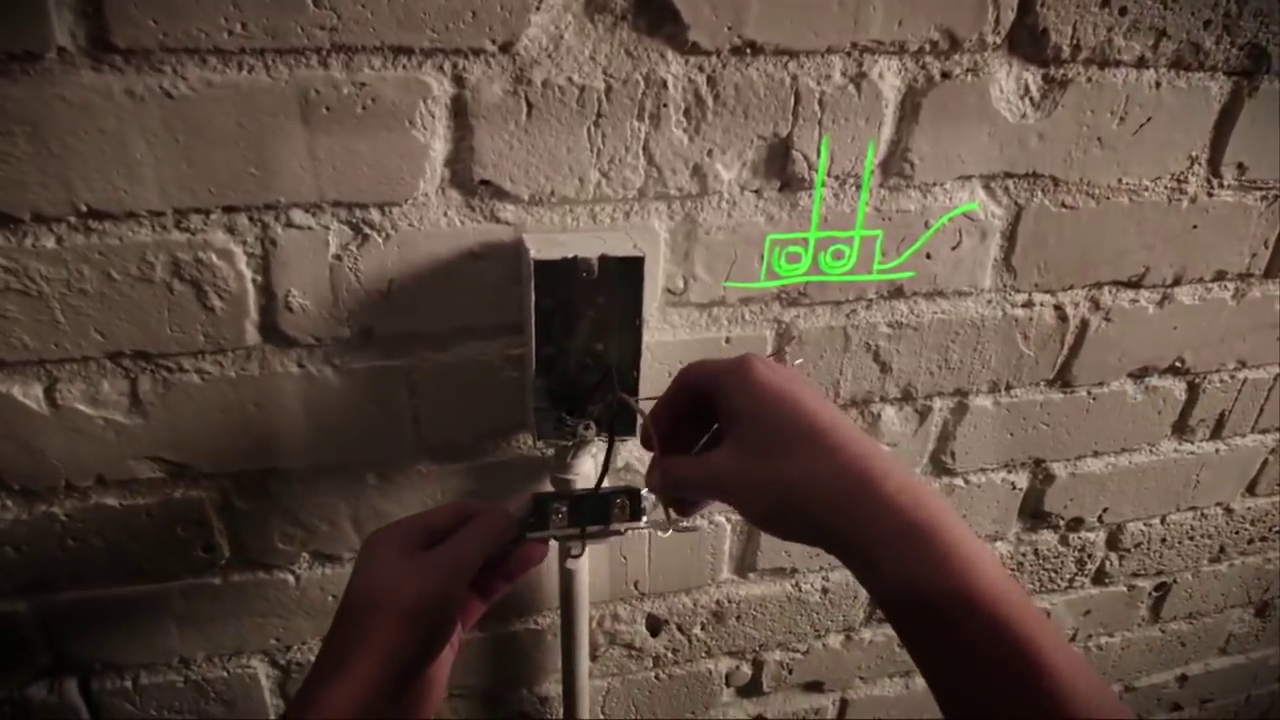
\includegraphics[width=0.4\textwidth]{\conclusion/fig/ar/hololens_fix2} \\
\multicolumn{2}{c}{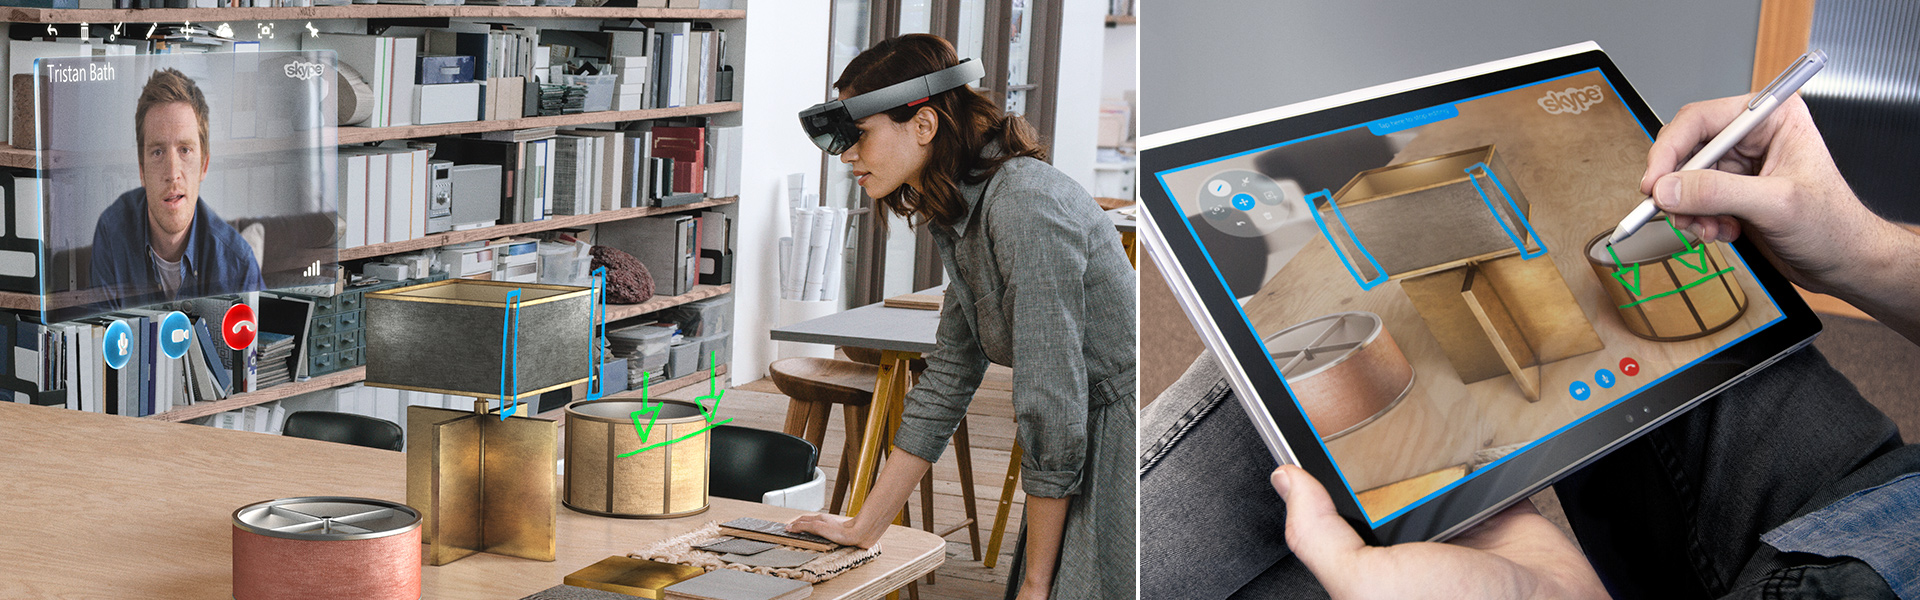
\includegraphics[width=0.82\textwidth]{\conclusion/fig/ar/hololens_skype} }
\end{tabular}
\caption{
  Microsoft's HoloLens~\cite{MicrosoftHoloLensSkype} has introduced an Augmented Reality application on providing real-time physical instructions from a remote instructor.
}
\end{figure*}

\section{Conclusion}
In this dissertation, we present video-based approaches designed for amateur users to produce and consume effective instructions from demonstrations. Using video and audio analysis techniques, our tools support recording, editing, and playback in a tutorial production process. We demonstrate results of our computer-generated tutorials from several domains, including software applications and physical activities. Our goal is to increase the quality of instructions created by tutorial authors and to support learners navigating and following the tutorials.

